% don't remove the folling lines, and edit the defintion of \main if needed
\documentclass[../report.tex]{subfiles}
\providecommand{\main}{..}
\IfEq{\jobname}{\currfilebase}{\AtEndDocument{\biblio}}{}
% until here

\begin{document}

\section{Invisible decays of the Higgs boson}\label{Sec:6Invisible}

\begin{center}
\textit{by Anne-Marie Magnan, Ben Nachman, Tania Robens and Tim Stefaniak}
\end{center} 

Invisible decays of the $125~\mathrm{\UGeV}$ Higgs boson are a generic prediction of new physics models that feature a light dark matter (DM) particle which couples directly or indirectly to the Standard Model Higgs field. The invisible branching ratio in the SM is very small (0.1\%) so any observable rate would be evidence for physics beyond the SM.  LHC searches for this signature require the Higgs boson to be produced in association with a taggable object, most importantly, a $Z$-boson, extra forward jets (as appearing in the vector boson fusion process), or a single high-$p_T$ jet. Furthermore, the invisible Higgs decay to the DM particles inevitably suppresses the branching fractions for the Higgs decays to SM particles. This --- along with possible model-dependent alterations of the Higgs couplings --- leads to a modification of the LHC Higgs signal rates of channels with SM final states with respect to their SM expectation, which can be probed with precision Higgs measurements. 

In so-called \emph{Higgs portal} models the SM Higgs field acts as a mediator between the visible SM sector and a hidden DM sector. {Commonly,} an additional symmetry {is introduced that} prohibits interactions of single hidden sector fields with SM fields, thus allowing only pair production of hidden sector particles and rendering the lightest hidden sector particle a stable DM candidate. 
The \emph{Higgs portal} and its generalisation to other non-SM Higgs bosons are found in many BSM scenarios (see e.g.~Refs.~\cite{McDonald:2008up,McDonald:2008ua,ArkaniHamed:2006mb,Profumo:2017ntc} and~\cite{Barger:2008jx,Cohen:2011ec,Englert:2011yb,Goudelis:2013uca,Bai:2012nv,Berlin:2015wwa} for models with and without supersymmetry). 

%{[\color{red} Add intro to experimental sections here!]}
The invisible decay of the Higgs is experimentally challenging because the missing transverse energy spectrum is relatively soft, where resolution and pileup effects are non-negligible.  The issues associated with pileup, both from pileup jets and from pileup-induced resolution degradation, will only become more severe beyond Run 3.  Significant recent advances in constituent-based pileup mitigation techniques will likely play a key role in maintaining and possibly improving the MET performance~\cite{Cacciari:2014gra,Bertolini:2014bba,Berta:2014eza,Komiske:2017ubm,Martinez:2018fwc}.  Furthermore, lepton identification and pileup jet rejection will both improve with the increased tracking acceptance planned by both ATLAS and CMS~\cite{Klein:2017nke,Collaboration:2283187,Collaboration:2283189,Collaboration:2293646,Collaboration:2017mtb,Collaboration:2285585}. Current analyses with $\sim 30$ fb$^{-1}$ place limits on the invisible branching ratio of the Higgs boson at about 20- 25\%~\cite{Khachatryan:2016whc,Aad:2015pla,Aaboud:2017bja,Aad:2015txa,Sirunyan:2018owy,Aaboud:2018sfi}.  The systematic uncertainty is about the same size as the statistical uncertainty; this means that the factor of 100 increase in statistics will not necessarily translate into an improvement by a factor of 10.  Early projections from ATLAS and CMS~\cite{CMS-PAS-FTR-16-002,ATL-PHYS-PUB-2013-014} predict limits that are a factor of 3-5 below the current result. The main limiting systematic uncertainty is from using $W\rightarrow l\nu$ to estimate the $Z\rightarrow \nu\nu$ in the dominant VBF channel. Advances in this theory input over the next decade could significantly improve the achievable precision. Already, CMS has shown that optimistic projections with reduced systematic uncertainties are realistic - the 2016 analysis~\cite{Sirunyan:2018owy} follows optimistic (reduced systematic uncertainties) scaling from the 2015 projection~\cite{CMS-PAS-FTR-16-002}.

Currently, the VBF production dominates the branching ratio limit.  This is because the VBF mode has a large cross-section (about 10\% of the total) and the main background $Z\rightarrow\nu\nu$ is qualitatively different (QCD production) from the same background in the $VH$ mode (EW production).  However, it is not clear which mode will dominate after Run 3, since there will be a non-trivial change in experimental conditions that will make both triggering and background rejection more difficult for both the VBF and $VH$ modes.  At the same time, there are many interesting opportunities to improve both channels from new detector capabilities (extended trackers and timing detectors) as well as new analysis techniques (e.g. quark/gluon tagging).

In this report we assess the prospects of probing \emph{Higgs portal} models directly with future searches for invisible Higgs decays, as well as indirectly with precision Higgs rate measurements, at the LHC in the high luminosity phase with $3~\mathrm{ab}^{-1}$. Furthermore, we shall highlight the complementarity between these two probes, as well as with other constraints, e.g.~with current and future limits from DM direct detection experiments and limits from LEP Higgs searches. Searches for invisible decays of the Higgs boson also have important implications for ``nearly invisible'' decays into neutral long-lived particles that are predicted by many models~\cite{Curtin:2018mvb}. Dedicated searches set much stronger limits~\cite{Aad:2015uaa,ATLAS:2016jza,Aaij:2016xmb,CMS:2014hka}, but the Higgs to invisible search is a model-independent constraint on all possibilities.  Projections for dedicated searches as well as proposals for dedicated detectors at the LHC complex~\cite{Chou:2016lxi,Gligorov:2017nwh,Gligorov:2018vkc} are not discussed in this section.

This contribution is organised as follows. We briefly review in Section~\ref{sec6:exp} the experimental input for the HL-LHC that we use in our study. In Section~\ref{sec6:effC} we first employ an effective description of the generic phenomenological Higgs features that appear in this class of models. We then focus on two specific realisations of the Higgs portal: in Section~\ref{sec6:minimalHP} we discuss the \emph{minimal Higgs portal}, where the SM Higgs field directly couples to an additional DM field through a quartic interaction; in Section~\ref{sec6:singletHP} we show results for the \emph{scalar singlet portal}, where an additional scalar singlet is acting as a mediator between the visible and hidden sector. We conclude in Section~\ref{sec6:conclusions}.


\subsection{Main channels for direct searches}\label{sec:expinp}

Given the VBF Higgs (VBFH) production presents the best sensitivity, this channel is chosen to investigate the sensitivity of the search with the HL-LHC~\cite{CMS-PAS-FTR-18-016}. The CMS phase-2 detector is simulated using Delphes~\cite{deFavereau:2013fsa} (fast parametrisation), with on average 200 interactions per bunch crossing.  A
cut-and-count approach similar to the one described in the analysis from Ref.~\cite{Sirunyan:2018owy} is used.

The VBF\PH signal samples are produced using \POWHEG
v2.0~\cite{Alioli:2010xd,Nason:2009ai} at next-to-leading order
in perturbative QCD, assuming 100\% branching ratio \BHinv of the Higgs boson
to invisible final states, and normalised using the SM inclusive Higgs
boson production cross sections provided in Ref.~\cite{deFlorian:2016spz}.  Full-simulation samples produced at 13\,\UTeV are used to derive the gluon-fusion contribution, applied as a fraction of the Delphes expected VBF\PH yields.

The main backgrounds are processes involving vector bosons (W,Z)
produced in association with jets, either through QCD or electroweak
(EWK) vertices.  Monte Carlo samples for these backgrounds are
generated at leading order using \MGvATNLO v2.2.2~\cite{Alwall:2014hca} interfaced with \PYTHIA v8.205~\cite{Sjostrand:2014zea} or higher. SM processes involving top quarks also contribute to the
background, and are simulated using a combination of the \POWHEG and \MGvATNLO generators. Backgrounds arising from QCD multi-jet events are simulated using \MGvATNLO interfaced with \PYTHIA, imposing a minimum threshold of 1000\,\UGeV on the di-jet mass at parton level.


The objects studied are as defined for the analysis in Ref.~\cite{Sirunyan:2018owy}, with extended coverage in pseudorapidity $\eta$. Electrons passing loose
identification criteria, with a transverse momentum p$_T>10$\,\UGeV, and $|\eta|<2.8$ are vetoed. Similarly, muons passing loose
identification criteria with p$_T>20$\,\UGeV and $|\eta|<3.0$ are
vetoed. Taus passing loose identification criteria with p$_T>20$\,\UGeV
and $|\eta|<2.8$ are vetoed. Jets are reconstructed using the
anti-k$_T$ algorithm~\cite{Cacciari:2008gp,Cacciari:2011ma} with a parameter size of
0.4.  The jets are required to have p$_T>30$\,\UGeV and $|\eta|<5.0$,
and are corrected for pileup effects using the ``Puppi''
algorithm~\cite{Bertolini:2014bba}.

 A b-tagging algorithm is used to tag jets that originate from decays
of B hadrons (b jets).  The algorithm uses a combination of vertexing
and timing information, and a working point with an efficiency of
around 60\% and a mis-tagging rate below 1\% is defined to identify b
jets.  Events containing any identified b jets are vetoed.

The leading and sub-leading jets in the event are required to have
p$_{T}>80$ and $40$\,\UGeV, respectively, and be in opposite hemispheres of
the detector. These two jets form the VBF di-jet pair, and further
requirements are applied on the invariant mass M$_{\text{jj}}$, and
their separations in pseudorapidity $|\Delta\eta_{\text{jj}}|>4.0$ and
azimuthal angle $|\Delta\phi_{\text{jj}}|<1.8$.

To reject the QCD multi-jet background, for which the transverse
missing energy arises from jet mis-measurements, the \METvec vector is
required to not be aligned with a jet using min$[\Delta\phi$(jet
\ptvec$>30$\,\UGeV, \METvec)]$>0.5$. The magnitude of the vector sum of
the p$_{T}$ of all jets with p$_{T}>30$\,\UGeV is defined as \MHT.

The analysis uses five non-overlapping event regions: the signal
region (SR) where events containing charged leptons ($\ell$, where
$\ell=\Pe$ or $\Pgm$) are vetoed, and four control regions (CR) with
exactly one electron or muon ($\PW\rightarrow\Pe\nu$ CR and
$\PW\rightarrow\Pgm\nu$ CR) or exactly two electrons or two muons
($\PZ\rightarrow\Pe\Pe$ CR and $\PZ\rightarrow\Pgm\Pgm$ CR).  In the
$\PW\rightarrow\Pe\nu$ and $\PW\rightarrow\Pgm\nu$ CRs, to further
reject QCD multi-jet backgrounds, the transverse mass, defined as
$\sqrt{2\pt^{\ell}\MET\left[1
- \cos{\Delta\phi(\ell,\METvec)}\right]}$, where p$_{T}^{\ell}$ is the
transverse momentum of the lepton and $\Delta\phi(\ell,\METvec)$ is
the azimuthal angle between the lepton momentum and $\METvec$ vectors,
is required to be less than 160\,\UGeV. In the W$\rightarrow$e$\nu$ CR a
selection on \MET$>60$\,\UGeV is also applied due to the higher QCD
multi-jet contamination than in the muon channel. In the
$\PZ\rightarrow\Pe\Pe$ and $\PZ\rightarrow\Pgm\Pgm$ CRs, the di-lepton
mass is required to be between 60 and 120\,\UGeV. To account for the
higher single-electron trigger thresholds that will be required at the
HL-LHC , the leading electron p$_{T}$ is required to be above 40\,\UGeV,
for both the $\PW\rightarrow\Pe\nu$ and $\PZ\rightarrow\Pe\Pe$ CRs.

The lower threshold on the \MET is varied from 130 to 400\,\UGeV in 10 to
50\,\UGeV steps. Likewise, the lower threshold on M$_{\text{jj}}$ is
varied from 1000 to 4000\,\UGeV in 100\,\UGeV steps. The statistical
uncertainty on the MC is considered to be negligible, assuming the
available MC samples will have at least 10 times the integrated
luminosity available in the data.  For each (\MET, M$_{\text{jj}}$)
selection, the yields are extracted in the four control regions and in
the signal region, and a likelihood is constructed as the product of
five Poisson terms, one per region.  Upper limits on the Higgs boson
production cross section times
\BHinv are placed at the 95\% CL using the CLs
criterion~\cite{Read:2002hq,Junk:1999kv,Dittmaier:2012vm}, with a profiled
likelihood ratio as the test statistic in which systematic
uncertainties are incorporated via nuisance
parameters~\cite{Chatrchyan:2013lba,CMS-NOTE-2011-005}. Asymptotic
formula are used to determine the distribution of the test statistic
under signal and background hypotheses~\cite{Cowan:2010js}.

The scenario considered for the systematic uncertainties is described
in table~\ref{tab:systs}, together with the systematic uncertainties that were 
considered in Ref.~\cite{Sirunyan:2018owy}, for comparison.

\begin{table}[ht]
  \centering
  {%\small
  \begin{tabular}{l|c|c}
    \hline
    Systematic & From Ref.~\cite{Sirunyan:2018owy} & This analysis \\
    \hline
    e-ID & 1\%(reco)$\oplus$1\%(idiso) & 1\% \\
    $\mu$-ID & 1\%(reco)$\oplus$1\%(id)$\oplus$0.5\%(iso) & 0.5\% \\
    \hline
    e-veto & 0.6\%(reco)$\oplus$1.5\%(idiso) & 1\% \\
    $\mu$-veto on QCD V+jets & 5\%(reco)$\oplus$5\%(id)$\oplus$2\%(iso) & 2\% \\
    $\mu$-veto on EWK V+2jets & 10\%(reco)$\oplus$10\%(id)$\oplus$6\%(iso) & 6\% \\
    $\tau$-veto & 1--1.5\% for QCD--EWK  & 0.5--0.75\% \\
    b-tag-veto & 0.1\% (sig) 2\% (top) & 0.05\% (sig) 1\% (top) \\
    \hline
    JES & 14\%(sig) 2\%(W/W) 1\%(Z/Z) & 4.5\%(sig) 0.5\%(W/W) 0.2\%(Z/Z) \\
    Integrated luminosity & 2.5\% & 1\% \\
    QCD multi-jet & 1.5\%  & 1.5\% \\
    \hline
    Theory on W/Z ratio & 12.5\% & 7\% \\
    ggH normalisation & 24\% & 20\% \\
    %QCDscale\_qqH & $^{+0.4\%}_{-0.3\%}$ & $^{+0.4\%}_{-0.3\%}$\\
    %QCDscale\_accept\_qqH	& 2\% & 1\% \\
    %pdf\_qqbar	        & 2\% & 1\% \\
    %pdf\_accept\_qqbar	& 1\% & 1\% \\
    %QCDscale\_ggH2in	& 40\%  & 20\% \\
    %QCDscale\_YR4\_ggH & $^{+4.6\%}_{-6.7\%}$   & $^{+2\%}_{-4\%}$ \\
    %pdf\_gg	&	3.2\%  & 1.5\% \\
    %UEPS	&	16.8\% & 9\% \\
    \hline
\end{tabular}
    } \caption{Impact on the signal and background yields from the
    different sources of systematic uncertainty considered in
    Ref.~\cite{Sirunyan:2018owy} and for the HL-LHC setup considered
    in this analysis.}  \label{tab:systs}
\end{table}

The analysis is expected to be systematics dominated, with the
dominant systematic uncertainties due to the muon and electron
efficiencies (e-ID and $\mu$-ID in table~\ref{tab:systs}), both in the control and signal regions, and the jet
energy scale (JES) evaluated for the signal (sig) or on the ratios of W and Z yields in signal and control regions (W/W and Z/Z in table~\ref{tab:systs}). In Ref.~\cite{Sirunyan:2018owy}, due to the limited size of the di-lepton
samples, the knowledge of the ratio of the cross sections of the W to
Z boson production was used as a constraint between the two
backgrounds, leading to an increased sensitivity. The theoretical
uncertainty on this ratio is set at 12.5\% from studies of missing
higher order QCD and EWK corrections~\cite{Sirunyan:2018owy}, for both
QCD and EWK production. Once 300\fbinv of data will be available, this
constraint will play a smaller role. It is expected that improvements
in theoretical calculations of the ratio will lead to half the current
theoretical uncertainty, namely 7\%.  This uncertainty is expected to
have an impact of at most 3--5\% for the selection with the largest
expected significance and is therefore neglected in the results
presented herein. However, the uncertainty will be relevant when
considering very tight selection criteria on \MET and M$_{\text{jj}}$,
i.e. when the statistical uncertainty in the CRs becomes dominant.


The most stringent upper limits are achieved in the regions with lower
thresholds on M$_{\text{jj}}$ and \MET of 2500\,\UGeV and 190\,\UGeV,
respectively, for the 3000\fbinv scenario. The minimum is rather flat
between M$_{\text{jj}}$ values of 2300 and 3000\,\UGeV, and between
\MET values of 170 and 220\,\UGeV, indicating limited impact from the size of the MC
samples. The upper limits degrade steeply as the \MET threshold
increases above 250\,\UGeV. The behaviour is similar for the 300 and
1000\fbinv scenarios, with best thresholds found at lower values
of \MET (170\,\UGeV) and M$_{\text{jj}}$ (1500 and 1800\,\UGeV respectively)
due to the interplay between the size of the control regions and the
systematic uncertainties.

Distributions in M$_{jj}$ for
the leading jet pair and \MET in the signal region are shown in
figure~\ref{fig:plotsdijetmet}, for an integrated luminosity of 3000 fb$^{-1}$. The
corresponding expected yields are shown in
table~\ref{tab:yieldsYR18}. The uncertainties shown represent the statistical 
uncertainties due to the limited size of the Delphes samples and are not used in the calculations
of the final limits.



 \begin{table}[h!]
     \centering

\begin{tabular}{l|c|c|c|c|c}
\hline
Process & SR          &     $\PW\rightarrow\Pe\nu$ CR      &   $\PW\rightarrow \Pgm\nu$ CR      &   $\PZ\rightarrow\Pe\Pe$ CR      & $\PZ\rightarrow \Pgm\Pgm$ CR  \\
\hline
VBF\PH & 47812 $\pm$ 584       & - & - & - & - \\
ggH & 972  & - & - & - & - \\
\hline
Z$\rightarrow \ell\ell$ (EWK) & 103 $\pm$ 8   & 398 $\pm$ 16 & 641 $\pm$ 20 & 1342 $\pm$ 30 & 1889 $\pm$ 35 \\
Z$\rightarrow \ell\ell$ (QCD) & 451 $\pm$ 90   & 944 $\pm$ 126 & 1048 $\pm$ 116 & 1347 $\pm$ 118 & 2297 $\pm$ 158 \\
\hline
Z$\rightarrow\nu\nu$ (EWK) & 15275 $\pm$ 358       & - & - & - & - \\
Z$\rightarrow\nu\nu$ (QCD) & 20968 $\pm$ 599       & - & - & - & - \\
\hline
W$\rightarrow\mathrm{e}\nu$ (EWK) & 3358 $\pm$ 62      & 18986 $\pm$ 146 & 72 $\pm$ 9 & 33 $\pm$ 6 & - \\
W$\rightarrow \mu\nu$ (EWK) & 3426 $\pm$ 62     & 7 $\pm$ 3 & 29360 $\pm$ 181 & - & 17 $\pm$ 4 \\
W$\rightarrow \tau\nu$ (EWK) & 3595  $\pm$ 64   & 55 $\pm$ 8 & 87 $\pm$ 10 & - & - \\
\hline
W$\rightarrow\mathrm{e}\nu$ (QCD) & 3994  $\pm$ 999   & 13376 $\pm$ 1656 & 170 $\pm$ 168 &  - & - \\
W$\rightarrow \mu\nu$ (QCD) & 6891 $\pm$ 1388  & - & 23322 $\pm$ 2096 & - & - \\
W$\rightarrow \tau\nu$ (QCD) & 4308 $\pm$ 938  & -       & -       & -       & - \\
\hline
Top & 2050 $\pm$  132   &  2171 $\pm$ 143 & 3735 $\pm$ 188 & 107 $\pm$ 36 & 130 $\pm$ 39 \\
QCD & -    & -       & -       & -       & -\\
\hline
\end{tabular}
\caption{Number of events expected after the final selection, M$_{\text{jj}}>2500$\,\UGeV and \MET$>190$\,\UGeV, with an integrated luminosity of 3000\fbinv. The uncertainties are the statistical uncertainties from the Delphes samples.}
\label{tab:yieldsYR18}
  \end{table}




\begin{figure}[htbp]
  \centering
    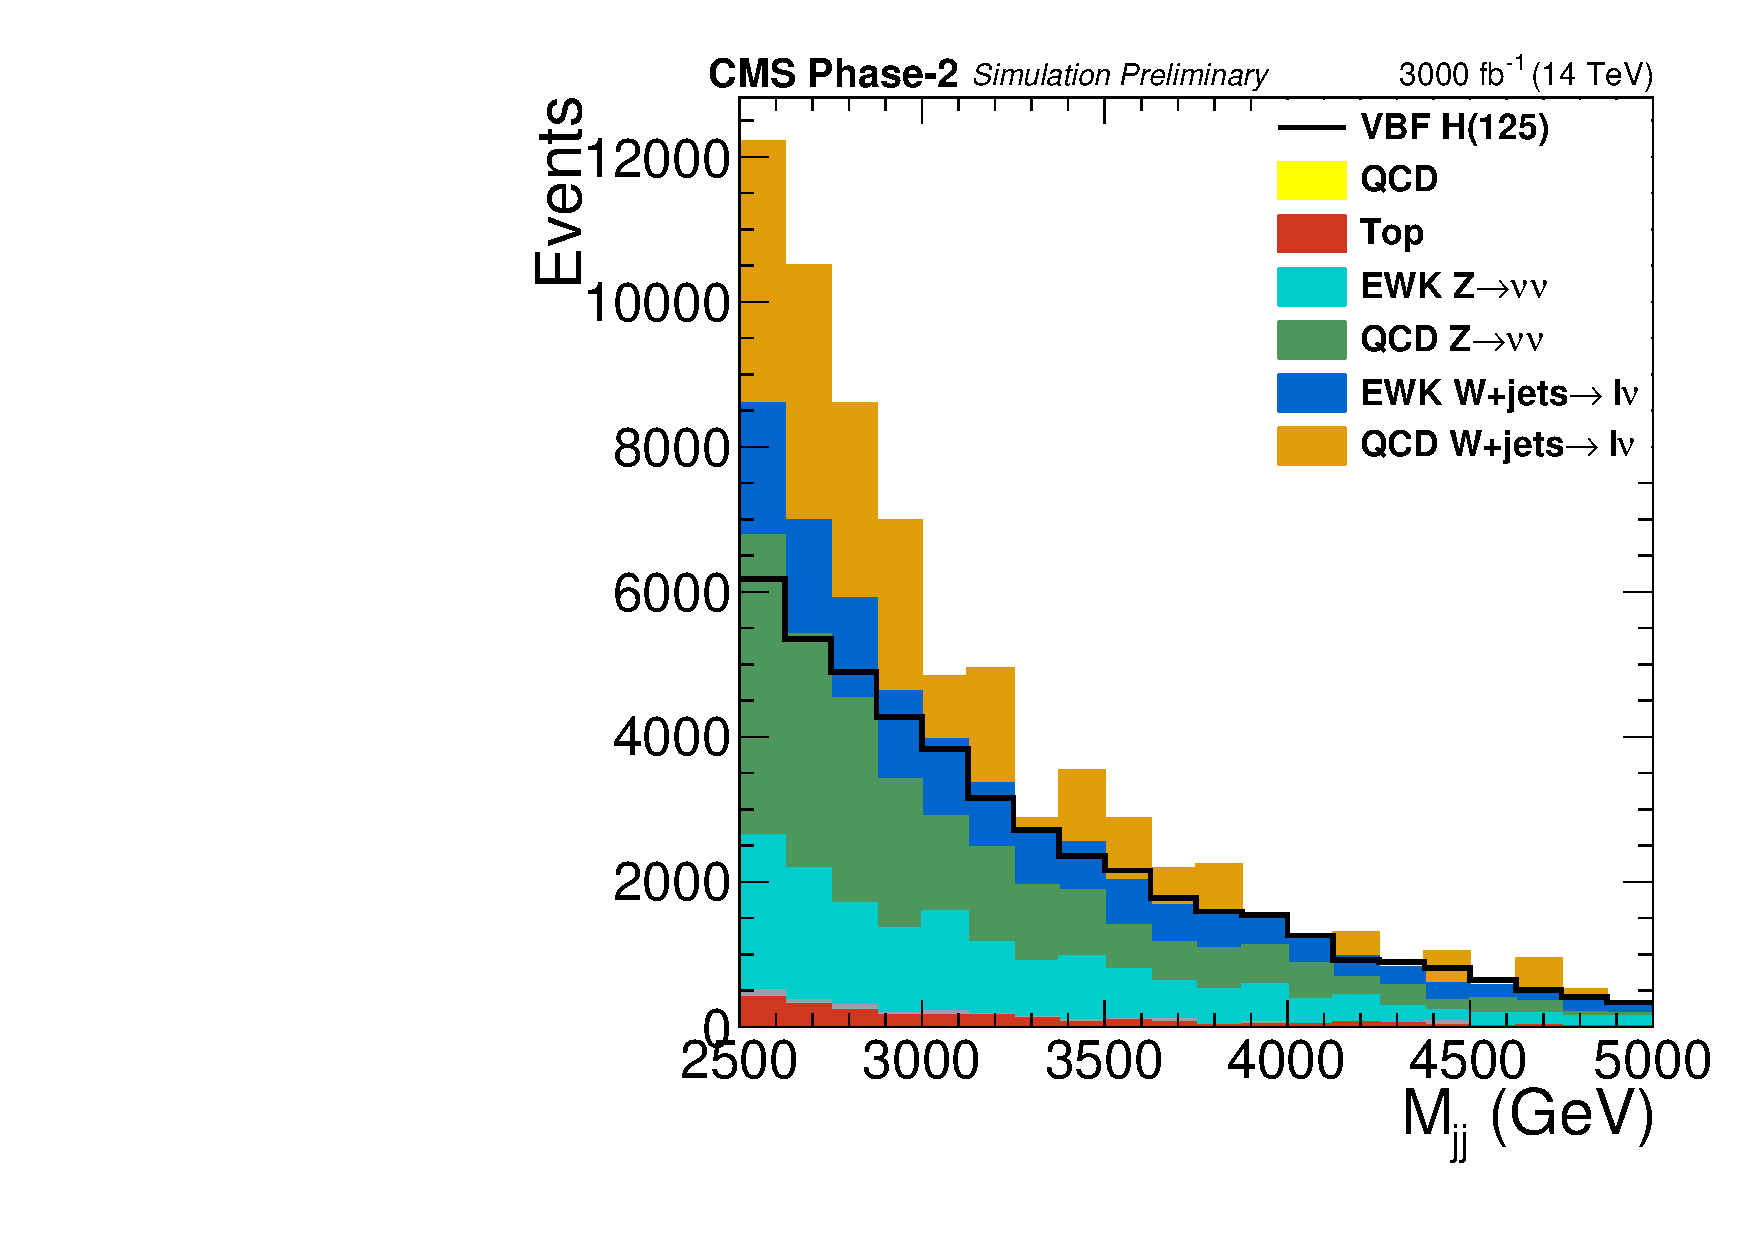
\includegraphics[width=0.49\textwidth]{\main/section6/plots/Mjj_200PU_cor}
    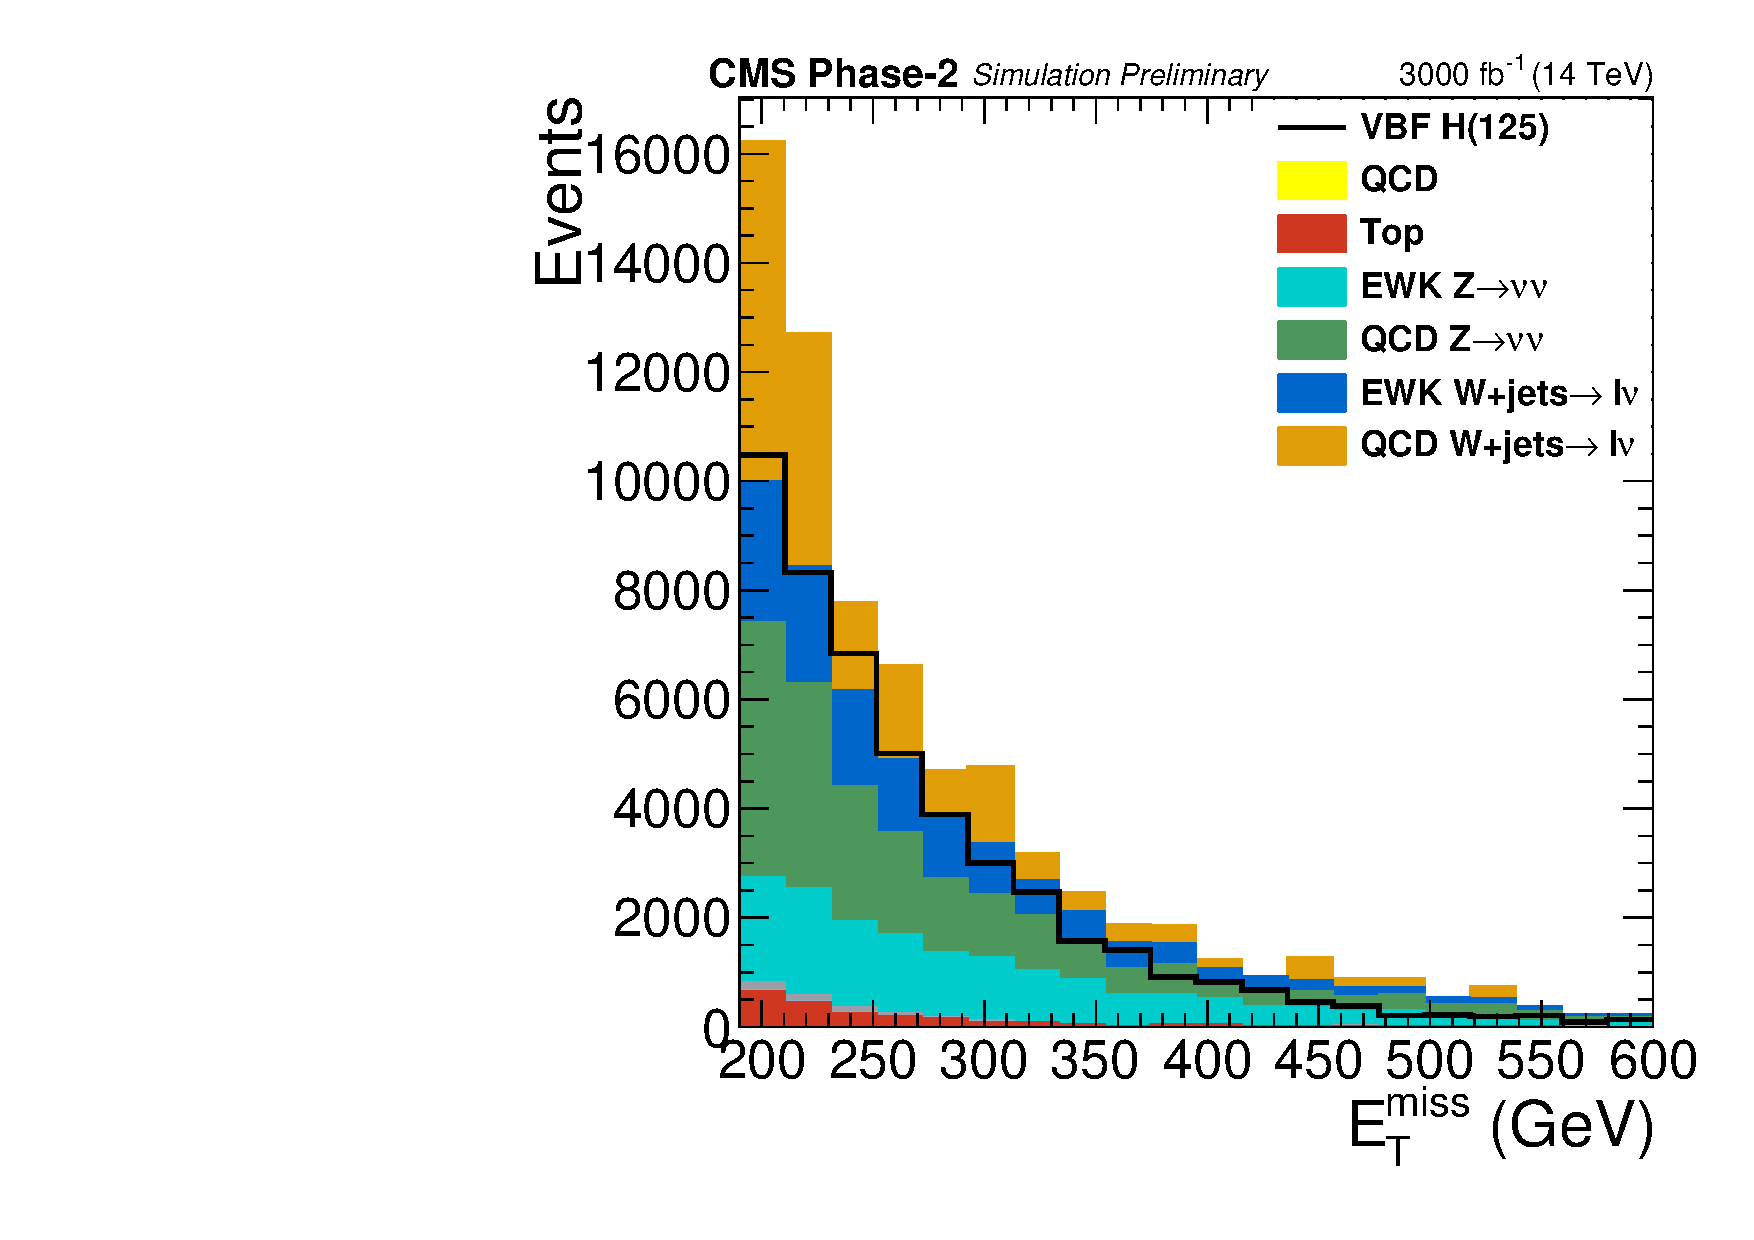
\includegraphics[width=0.49\textwidth]{\main/section6/plots/metnolep_200PU_cor}
\caption{Distributions of M$_{jj}$ (left) and \MET (right) in the signal region for the final selection, M$_{jj}>2500$\,\UGeV and \MET$>190$\,\UGeV~\cite{CMS-PAS-FTR-18-016}.}
  \label{fig:plotsdijetmet}
\end{figure}

The 95\% CL upper limits for an integrated luminosity of 3000\fbinv
are shown in figure~\ref{fig:1Dlimits}, left, as a function of the
thresholds applied on \MET assuming the MC statistical uncertainties
are negligible, for the final selections described above; similar results have been found in Ref.~\cite{Biekotter:2017gyu}, including a comparison with the ZH channel. In the best
case, the lowest 95\% CL limit on \BHinv, assuming Standard Model
production, is expected to be at 3.8\%, for thresholds values of
2500\,\UGeV (190\,\UGeV) on the di-jet mass (\MET). If the \MET resolution
was to be a factor of 2 worse, the re-optimisation of the selection
leads to minimum thresholds of 1800\,\UGeV (250\,\UGeV) on the di-jet mass
(\MET), but a similar 95\% CL limit. The limits are shown for
different integrated luminosities in figure~\ref{fig:1Dlimits}, right.


\begin{figure}[htbp]
  \centering
    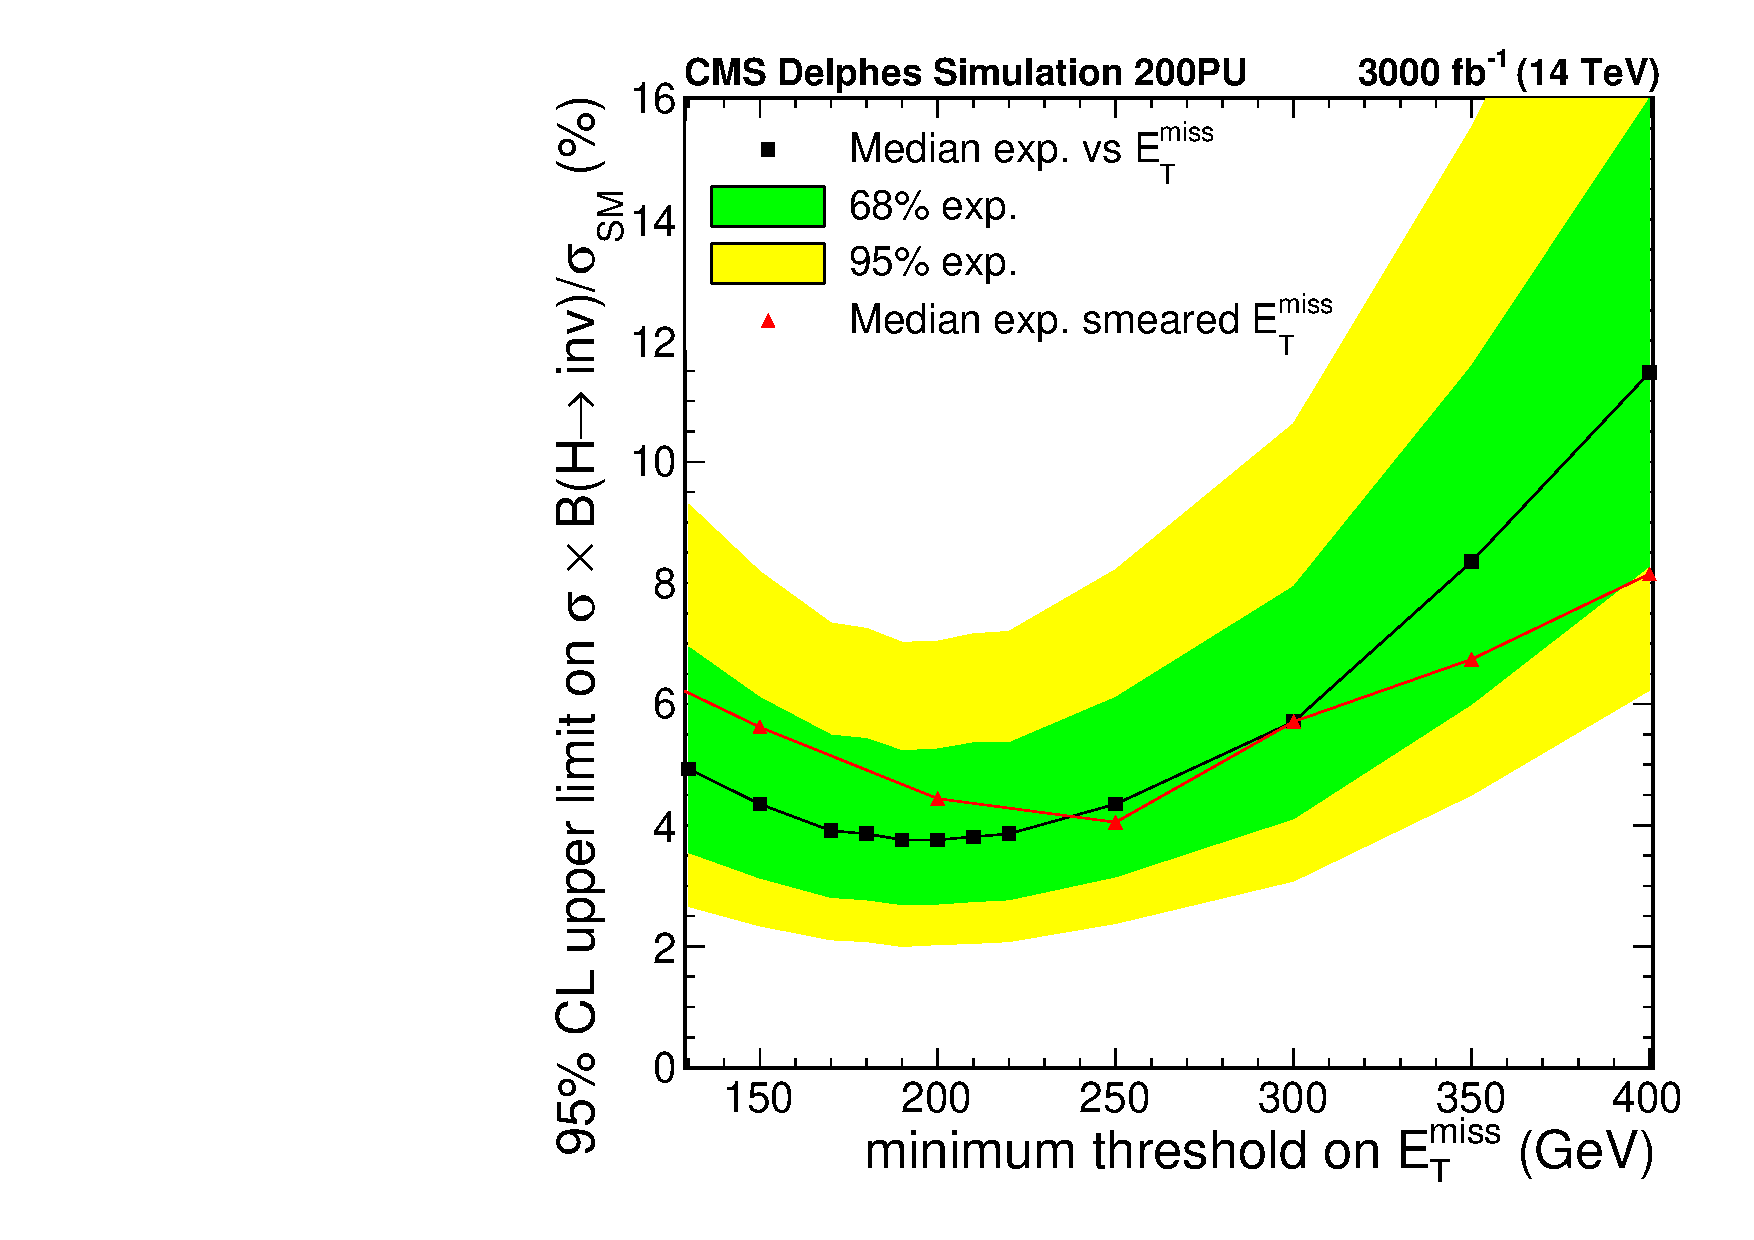
\includegraphics[width=0.49\textwidth]{\main/section6/plots/1DlimitMET_forPAS_noMHT}
    \hfill
    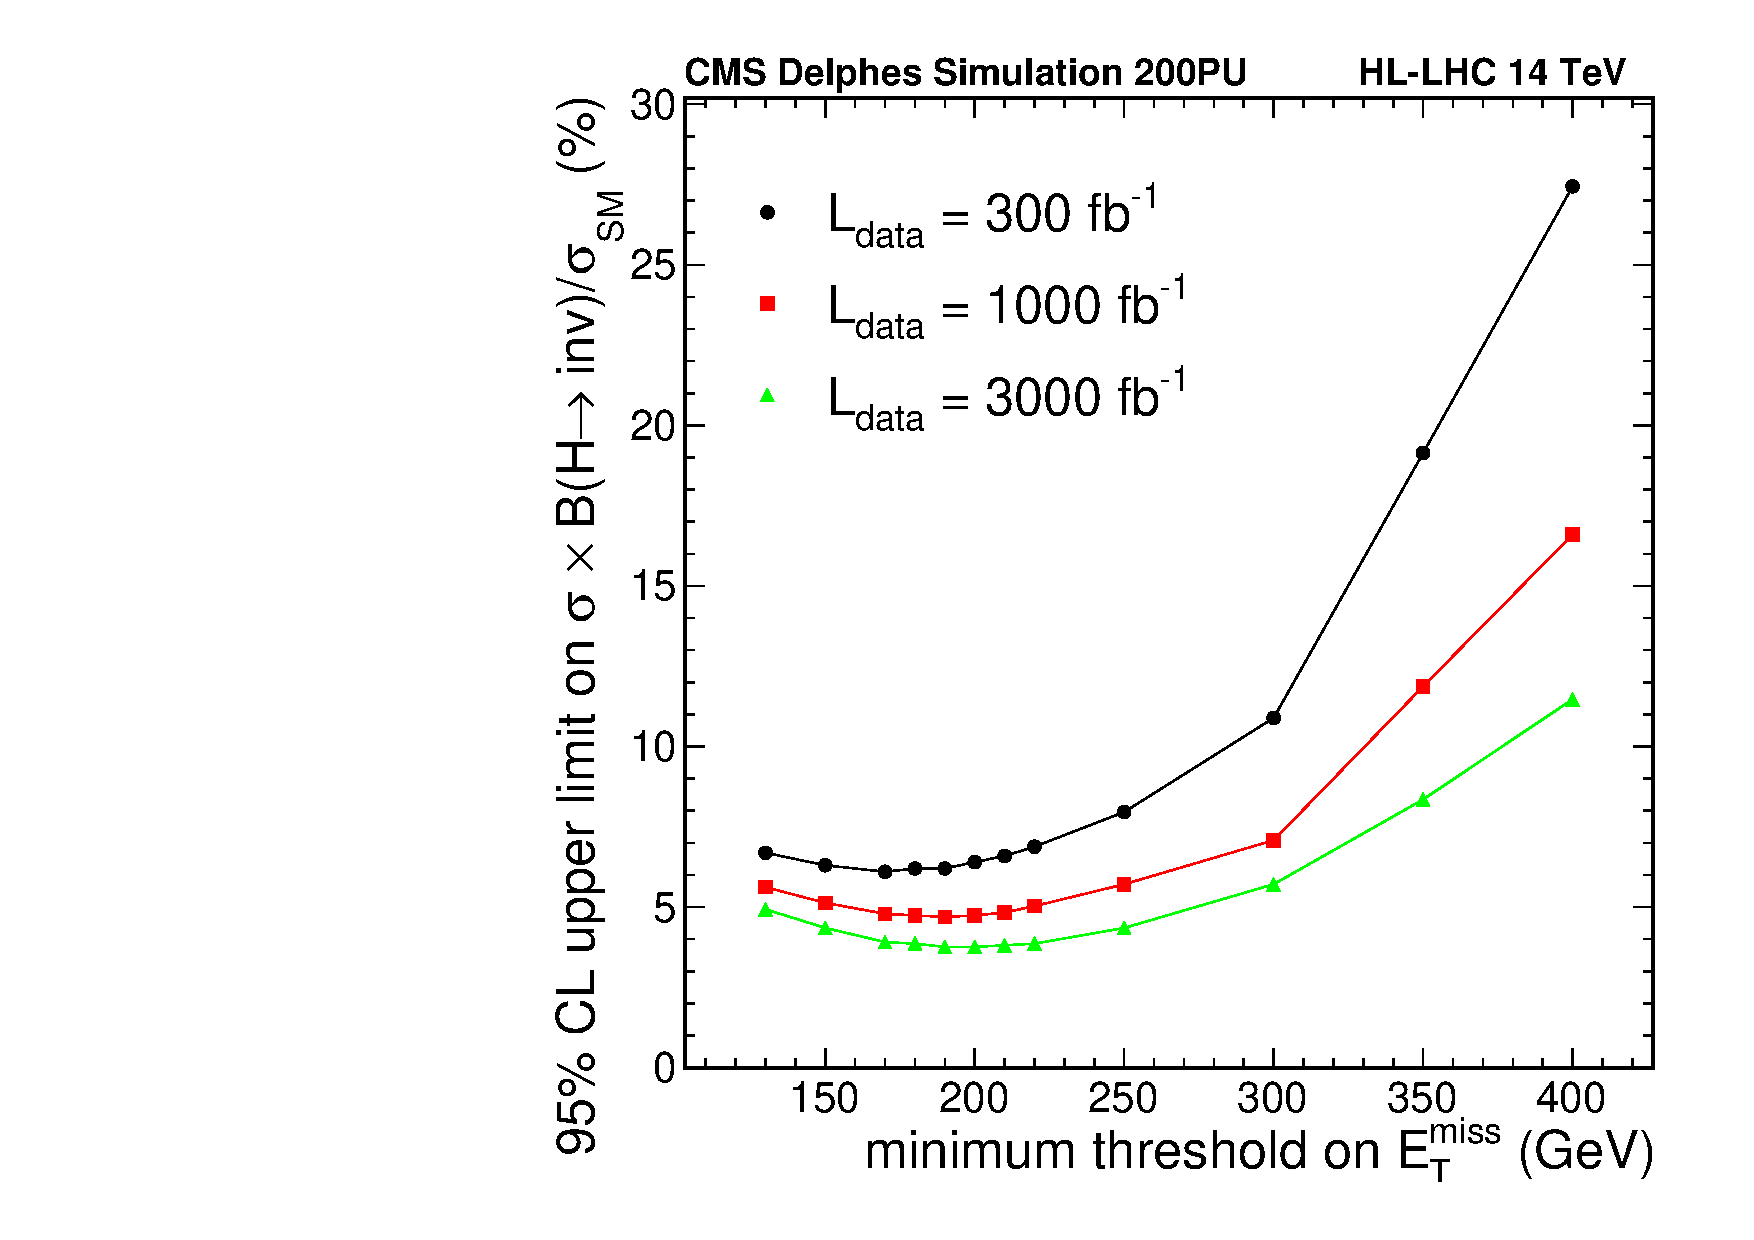
\includegraphics[width=0.49\textwidth]{\main/section6/plots/1DlimitvsMET_mcScenario4}
\caption{Left: 95\% CL limits on \BHinv as a function of the minimum threshold on \MET, for M$_{\text{jj}}>2500$\,\UGeV and an integrated luminosity of 3000\fbinv ~\cite{CMS-PAS-FTR-18-016}. Right: 95\% CL limits for scenarios with different integrated luminosities.}
  \label{fig:1Dlimits}
\end{figure}


The performance of pileup mitigation techniques will have a significant impact on the projected sensitivity for the final VBF result. ATLAS has conducted a study to show the impact of pileup jets on the invisible Higgs branching ratio limit in the VBF channel~\cite{ATL-PHYS-PUB-2018-038} using full detector simulations based on Geant4\cite{Agostinelli:2002hh,Allison:2006ve} and the complete detector simulation and event reconstruction. The branching ratio limit can vary by a factor of 4 when no explicit pileup jet mitigation is used to the case when truth information is used to remove all pileup jets. Therefore, the development of improved pileup jet mitigation will be an important development to empower the invisible Higgs decay analyses in the future.





\subsection{Interpretation and combination with precision Higgs boson measurements}
\subsubsection{Experimental input}
\label{sec6:exp}
{For the VBF production channel, the projected HL-LHC limit on the invisible Higgs decay rate from the CMS experiment amounts to $4\%$, see Section~\ref{sec:expinp}. For the $VH$ production channel ATLAS projected a limit of around $8\%$ in 2013}~\cite{ATL-PHYS-PUB-2013-014}.
Assuming ATLAS (CMS) performs equally well as CMS (ATLAS) in the $\text{VBF}$ ($VH$) channel, and neglecting possible correlations of experimental and theoretical uncertainties~\cite{CMS-PAS-JME-15-001}, a combination of these limits results in
\begin{align}\label{eq:brinvcombi}
\left(\mu_{\text{VBF},VH} \cdot \BRHinv \right)^\text{HL-LHC} \le 2.5\%,
\end{align}
where $\mu_{\text{VBF},VH}$ is a common signal strength modifier of the VBF and $VH$ production cross sections. In our theory interpretations below, we take Eq.~\eqref{eq:brinvcombi} as a benchmark value for the prospective ATLAS and CMS combined limit on $\BRHinv$.


We implemented the ATLAS and CMS HL-LHC projections for Higgs signal strength measurements for the individual production times decay modes (see Section~\ref{sec2:exp_combination}) into the code \texttt{Higgs\-Signals}~\cite{Bechtle:2013xfa,Bechtle:2014ewa}, including the corresponding correlation matrices.
We consider the projections for both future scenarios S1 (with Run~2 systematic uncertainties) and S2 (with YR18 systematic uncertainties)~\cite{HLHELHCCommonSystematics}, see Sec.~\ref{sec:expcomb_prodtimesdecay}, Tab.~\ref{tab:summary_A1_5PD}.
Note that correlations of theoretical rate uncertainties between the future ATLAS and CMS measurements are taken into account in our fit via \texttt{HiggsSignals}. 

We furthermore study the impact of a future electron-proton collider option (LHeC) at CERN~\cite{AbelleiraFernandez:2012cc,uta,uta2,Zimmermann:2651305}, assuming a $60~\mathrm{\UGeV}$ electron beam, a $7~\mathrm{\UTeV}$ proton beam and an integrated luminosity of $1~\mathrm{ab}^{-1}$. We implemented the prospective signal strength measurements at the LHeC presented in Ref.~\cite{uta} into \texttt{HiggsSignals}.\footnote{In addition to the experimental precision quoted in Ref.~\cite{uta} we assume a theoretical uncertainty of $1\%$ ($1.5\%$) on the charged (neutral) current production cross section, as well as a $1\%$ luminosity uncertainty.} The projected limit on the invisible Higgs decay rate is around $5\%$~\cite{uta,Tang:2015uha,kuzeLHeC,bc1,bc2,uta2} \footnote{Optimisation of the signal selection, advanced background estimation techniques and details of the detector design may improve this limit down to about $(3-4)\%$~\cite{Utacommunications}.}.
In combination with the above CMS and ATLAS projections, we obtain
\begin{equation*}
\left(\mu_{\text{VBF},VH,\text{NC}} \cdot \text{BR}_\text{inv}\right)^{\text{HL-LHC}\oplus\,\text{LHeC}}\,\leq\,2.25\%
\end{equation*}
as upper limit on the branching ratio of an invisible Higgs decay mode. {Here, {we assume} the common signal strength modifier $\mu$ also applies to the neutral current (NC) Higgs production cross section at the LHeC.}


\subsubsection{Effective description of Higgs portal models}
\label{sec6:effC}

In this section we discuss the HL-LHC prospects in the context of an effective parametrisation of Higgs rate modifications that are commonly predicted by Higgs portal models, using the coupling scale factor ($\kappa$) framework~\cite{Heinemeyer:2013tqa} (see also Section \ref{sec2:exp_kappa}).  Herein, the scale factors $\kappa_X$ ($X = W, Z, g, \gamma, b, \tau, \dots$) are introduced for every relevant Higgs coupling to SM particle $X$. The partial widths and cross sections associated with these Higgs couplings are then rescaled by $\kappa^2_X$ (see Refs.~\cite{Heinemeyer:2013tqa,Bechtle:2014ewa} for more details). In addition, we treat the branching fraction for invisible Higgs decays, $\BRHinv$, as free parameter.

In particular, we investigate two scenarios for the Higgs coupling modifications:
\begin{enumerate}
\item[(\emph{i})] a universal scale factor for all Higgs couplings to SM particles, $\kappa \equiv \kappa_X$ ($X = W, Z, g, \gamma, b, \tau, \dots$);
\item[(\emph{ii})] additional free parameters $\kappa_g$ and $\kappa_\gamma$ that rescale the loop-induced Higgs couplings to gluons and photons, respectively. The remaining (tree-level) Higgs couplings to SM particles are again rescaled universally with $\kappa \equiv  \kappa_X$ ($X = W, Z, b, \tau, \dots$).
\end{enumerate}

\begin{figure}
\centering
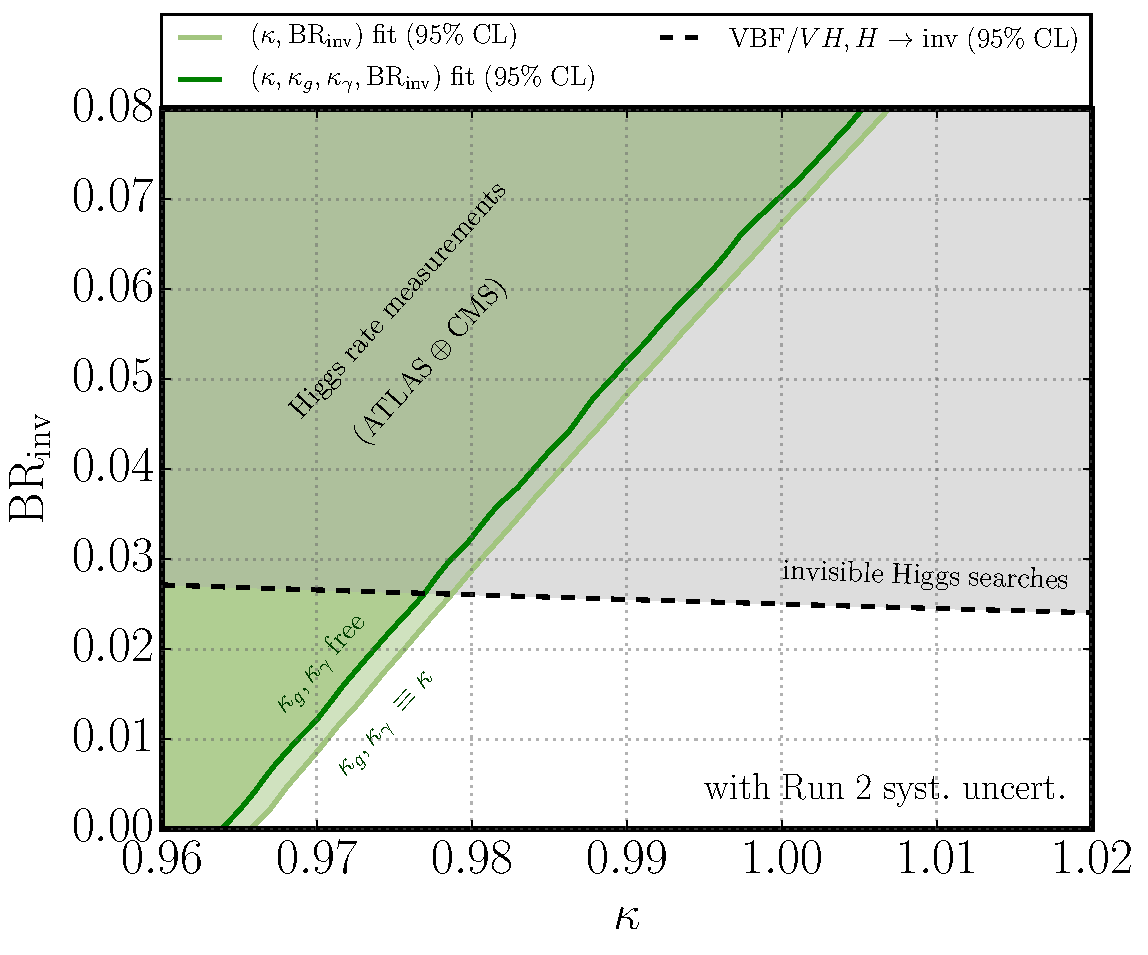
\includegraphics[width=0.49\textwidth]{\main/section6/plots/kappa_BR_S1}
\hfill
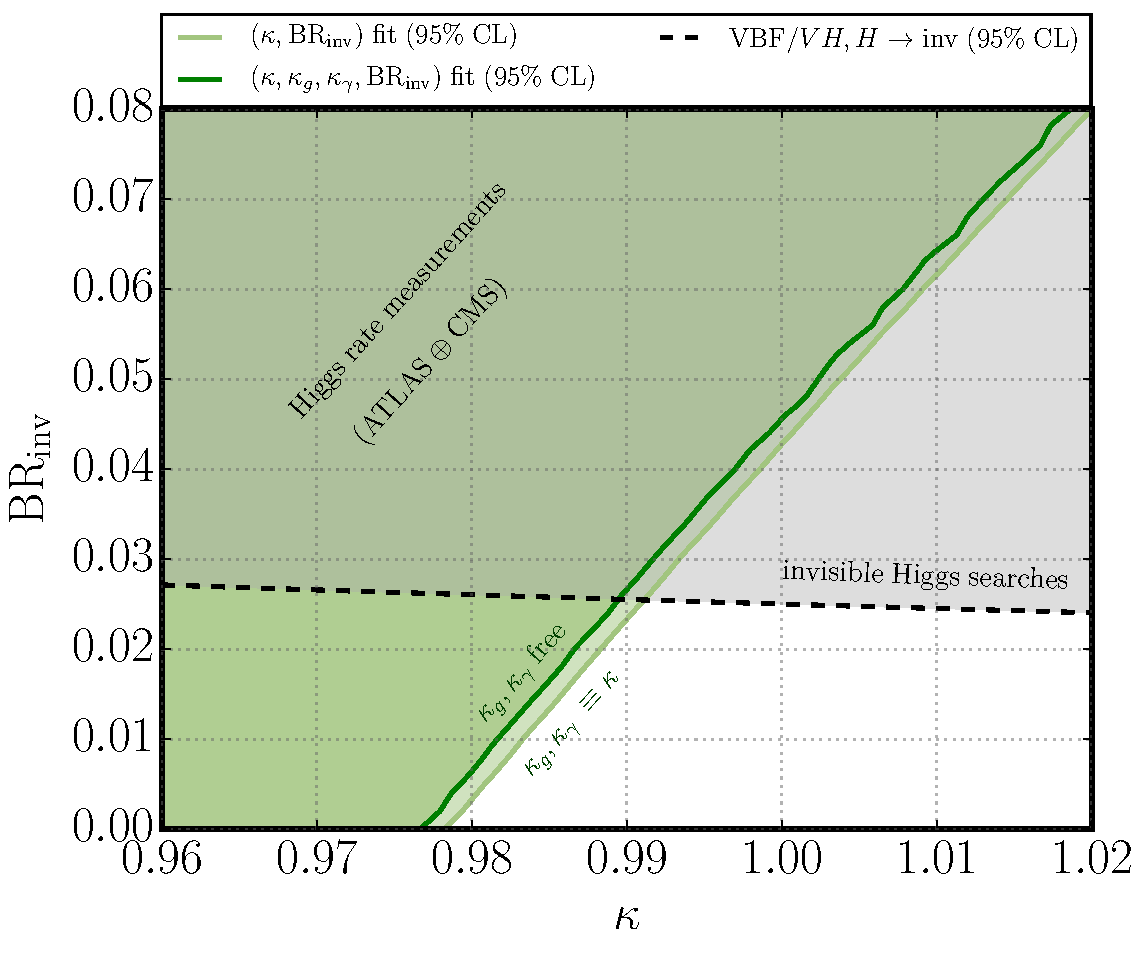
\includegraphics[width=0.49\textwidth]{\main/section6/plots/kappa_BR_S2}\\
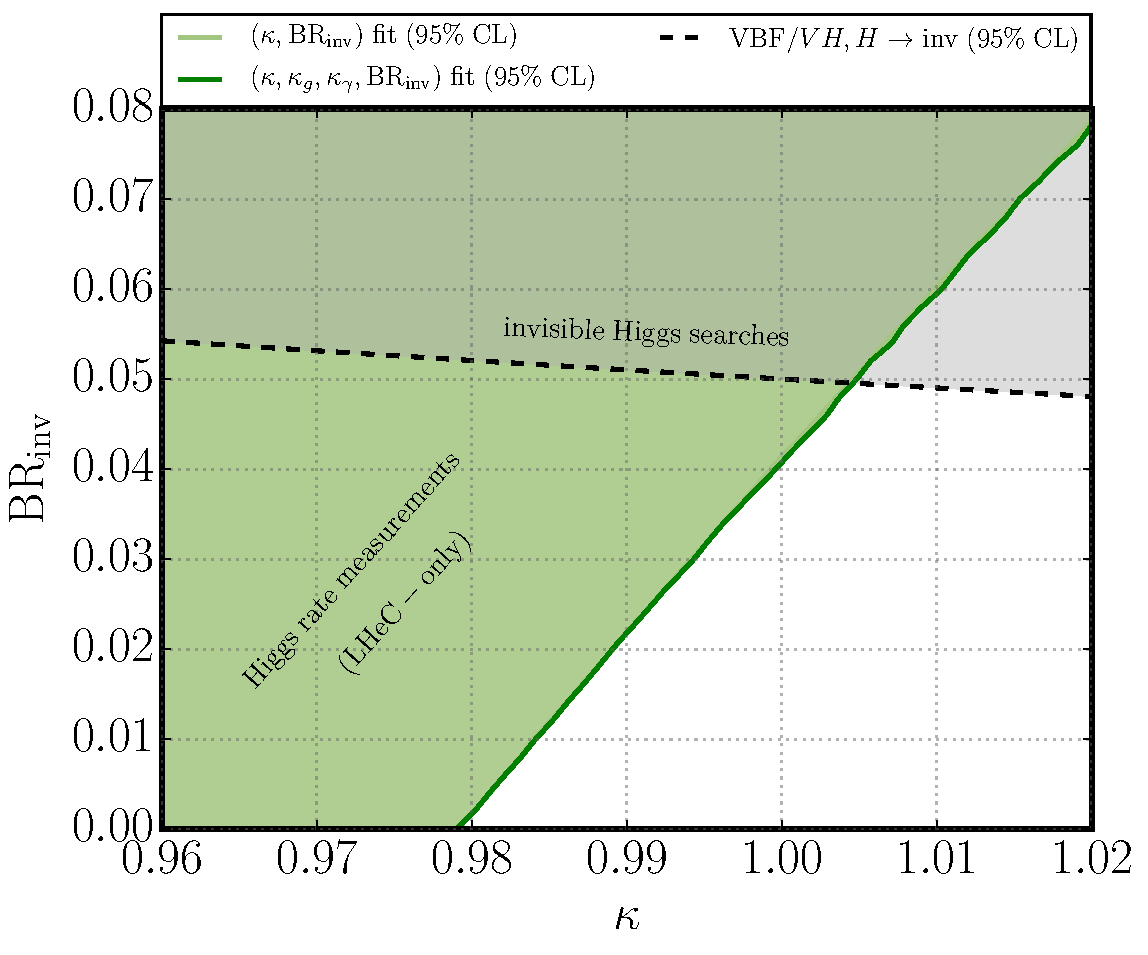
\includegraphics[width=0.49\textwidth]{\main/section6/plots/kappa_BR_LHeC_BRinv0p05}
\hfill
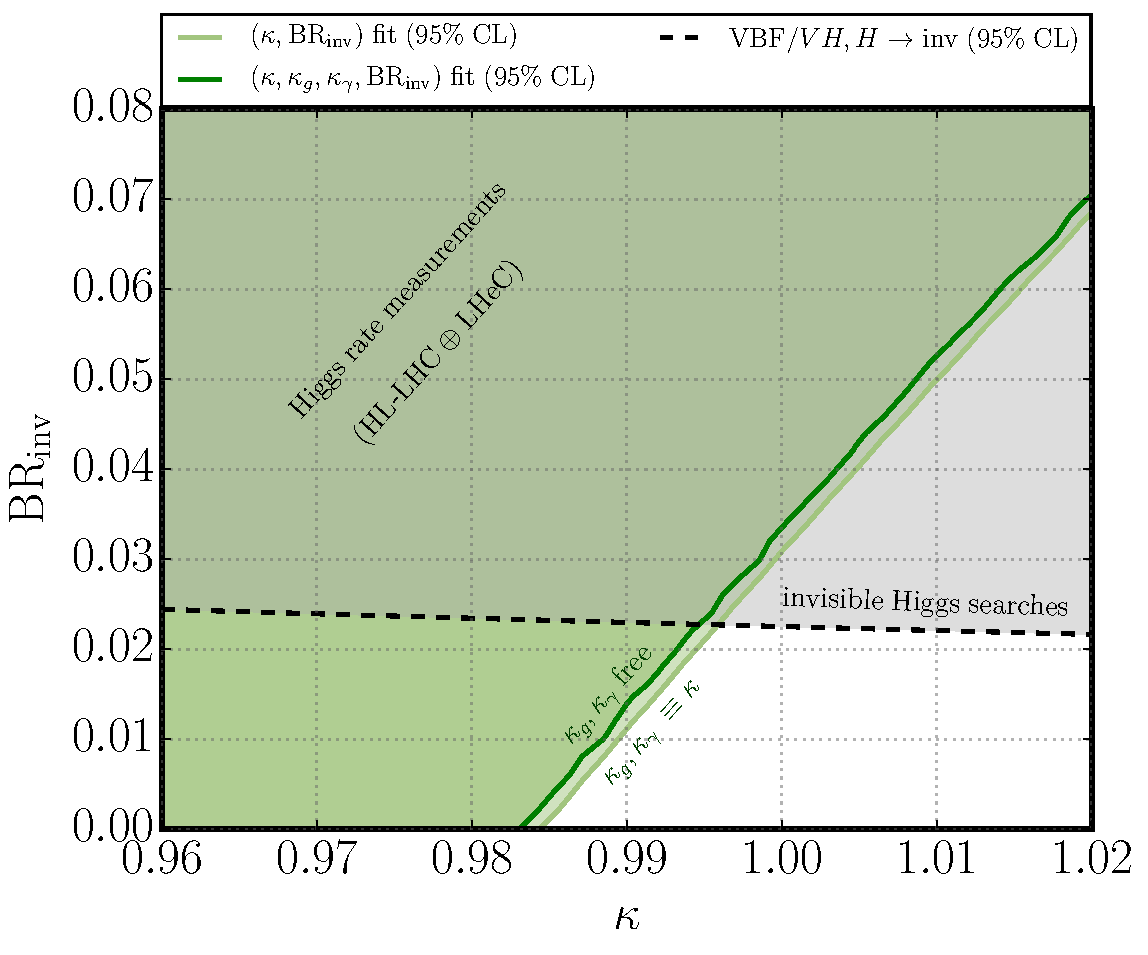
\includegraphics[width=0.49\textwidth]{\main/section6/plots/kappa_BR_LHeC_HLLHCS2_BRinv0p0225}
\caption{Projected $95\%~\mathrm{C.L.}$ limit in the $(\kappa, \BRHinv)$ plane inferred from Higgs rate measurements (\emph{green regions}) and direct invisible Higgs searches (\emph{black dashed line}) at the HL-LHC and LHeC. We show results for the two future HL-LHC scenarios S1 [with Run~2 systematic uncertainties] {\sl (top left)} and S2 [with YR18 systematic uncertainties] {\sl (top right)} (see text for details), as well as for the LHeC {\sl (bottom left)} and the combination of LHeC and HL-LHC~[S2] {\sl (bottom right)}. The light green area shows the limit from Higgs rates obtained by assuming no new physics contributions to the loop-induced Higgs couplings to gluons and photons, $\kappa = \kappa_g = \kappa_\gamma$, whereas for the dark green area $\kappa_g$ and $\kappa_\gamma$ are marginalised free parameters.}
\label{fig:effC}
\end{figure}

We employ the program \texttt{HiggsSignals}~\cite{Bechtle:2013xfa,Bechtle:2014ewa} to perform a $\chi^2$ fit to the projected HL-LHC {and/or LHeC} Higgs rate measurements (see Section~\ref{sec6:exp})  in each scenario. The resulting future $95\%~\mathrm{C.L.}$ limit is shown in Fig.~\ref{fig:effC} as a light and dark green area for scenario (\emph{i}) and (\emph{ii}), respectively. {The \emph{top panels} display the HL-LHC projections for future scenarios S1 [with Run~2 systematic uncertainties] (\emph{left}) and S2 [with YR18 systematic uncertainties] (\emph{right}), while the \emph{bottom panels} show the projections for LHeC (\emph{left}) and the combination of LHeC with HL-LHC S2 measurements (\emph{right}).} {In Tab.~\ref{tab:effC_limits} we summarise the lower limits on the Higgs signal strength of channels with SM final states, $\kappa^2 (1-\BRHinv)$, as well as the upper limits on the invisible Higgs decay rate, $\mathrm{BR}_\text{inv}$, assuming SM Higgs coupling strengths ($\kappa \equiv 1$), for the four future collider scenarios and for the two global fit scenarios.} Note that these results do not strictly require the additional Higgs decay mode to yield an invisible final state.

\begin{table}
\centering
\begin{tabular}{ l |  l | cccc}
\hline
fit setup &  quantity   & HL-LHC S1   & HL-LHC S2   & LHeC	  & LHeC $\oplus$ HL-LHC S2 \\
\hline
\multirow{2}{*}{$(\kappa, \mathrm{BR}_\text{inv})$}                         &  $\kappa^2 (1-\BRHinv)$ &  $\ge 0.933$ & $\ge 0.958$ & $\ge 0.959$  & $\ge 0.967$ \\
                                                                            &  $\BRHinv$ ($\kappa\equiv 1$) & $\le 6.7\%$ & $\le 4.2\% $ & $\le 4.1\%$ & $\le 3.3\%$\\
\hline									  
\multirow{2}{*}{$(\kappa, \kappa_g, \kappa_\gamma,  \mathrm{BR}_\text{inv})$}   &  $\kappa^2 (1-\BRHinv)$ & $\ge0.930$ &  $\ge0.954$ & $\ge0.959$ & $\ge0.966$\\
                                                                                &   $\BRHinv$ ($\kappa\equiv 1$) & $\le7.0\%$ & $\le4.6\%$ & $\le4.1\%$ & $\le3.4\%$\\

\hline
\end{tabular}
\caption{{Comparison of prospective $95\%~\mathrm{C.L.}$ limits on the Higgs signal strength for SM final states, $\kappa^2(1-\mathrm{BR}_\text{inv})$, and the invisible Higgs decay rate, $\mathrm{BR}_\text{inv}$ (assuming SM Higgs couplings, $\kappa =1$), for HL-LHC scenarios S1 and S2, LHeC, and the combination of LHeC and HL-LHC (assuming scenario S2). First (second) row shows the results obtained in the fit parametrisation (\emph{i}) [(\emph{ii})].}}
\label{tab:effC_limits}
\end{table}


These results are compared in Fig.~\ref{fig:effC} with the prospective future limits from direct searches for invisible Higgs decays (see Section~\ref{sec6:exp}). At the HL-LHC, assuming scenario S1 (S2), direct invisible Higgs searches are more sensitive than Higgs rates if deviations from the SM Higgs couplings are small, $\Delta \kappa \equiv 1- \kappa \lesssim 2~(1)\%$. For larger suppression of the Higgs couplings the Higgs rates will provide the strongest constraint. In contrast, if we allow for an enhancement of the Higgs couplings, $\kappa > 1$, the invisible Higgs searches will provide the strongest constraint (besides other bounds on the Higgs total decay width, see Sec.~\ref{sec5}).



At the LHeC the prospective indirect Higgs rate constraints are comparable to the HL-LHC S2 prospects, reaching a precision of $\Delta \kappa \lesssim (2.1-2.3)\%$ independently of the invisible Higgs decay rate, in both fit parametrisations considered here.\footnote{The complementarity of LHeC and HL-LHC Higgs rate measurements is much stronger in more general coupling fit setups, e.g., when independent scale factors for the Higgs-$W$-$W$ and Higgs-$Z$-$Z$ couplings are considered~\cite{uta}.} On the other hand, the direct invisible Higgs searches at the LHeC are weaker than at the HL-LHC. In combination with the HL-LHC (assuming future scenario S2), the bounds from the Higgs rates can further be improved to coupling deviations of $\Delta \kappa \lesssim1.7\%$. 

{Compared with the sensitivity of Higgs rate measurements during Run~1 of the LHC~\cite{Khachatryan:2016vau} to the invisible decay rate, $\BRHinv \lesssim \mathcal{O}({20\%})$} (at $95\%~\mathrm{C.L.}$), we find that the sensitivity improves by roughly a factor of $3$--$5$  at the HL-LHC (depending on the evolution of systematic uncertainties). In combination with LHeC results we expect the indirect limit to improve by a factor of up to $6$.



\subsection{Higgs portal interpretations}

\subsubsection{Minimal Higgs Portal}
\label{sec6:minimalHP}

In the minimal Higgs portal model, we impose a quartic interaction of the SM Higgs doublet field $H$ with the DM field, which could be either a scalar ($S$)~\cite{Silveira:1985rk}, a vector ($V^\mu$)~\cite{Lebedev:2011iq} or a fermion ($\chi$)~\cite{Kim:2006af} (see Refs.~\cite{Kanemura:2010sh,Djouadi:2011aa} for a comprehensive overview):
\begin{align}
\mathcal{L} &\supset -\tfrac{1}{4} \lambda_{hSS} H^\dagger H S^2 \qquad (\mbox{scalar~DM}) \quad \mbox{or} \label{eq:scalarDM}\\
\mathcal{L} &\supset +\tfrac{1}{4}  \lambda_{hVV} H^\dagger H V_\mu V^\mu \qquad (\mbox{vector~DM}) \quad \mbox{or} \label{eq:vectorDM}\\
\mathcal{L} &\supset -\tfrac{1}{4}  \tfrac{\lambda_{h\chi\chi}}{\Lambda} H^\dagger H \bar{\chi} \chi \qquad (\mbox{fermion~DM}), \label{eq:fermionDM}
\end{align}
respectively. Besides these operators the Lagrangian contains an explicit mass term of the DM field, allowing us to use the mass of the DM particle, $M_\text{DM}$, as a free model parameter. In addition, the Lagrangian $\mathcal{L}$ contains DM self-interaction operators, however, these are irrelevant to our study.


If DM is light, $M_\text{DM} < M_H /2 \simeq 62.5\UGeV$, the above interactions lead to the invisible Higgs decay into two DM particles. An upper limit on $\BRHinv$ can therefore be translated into an upper limit on the portal coupling $\lambda$ of above operators, Eqs.~\eqref{eq:scalarDM}-\eqref{eq:fermionDM}, depending on $M_\text{DM}$.  At the same time, the portal coupling $\lambda$ governs the DM phenomenology. For DM masses $M_\text{DM} \lesssim M_H/2$ the relic abundance of the DM particles is driven by the $s$-channel annihilation through the exchange of the Higgs boson.\footnote{Assuming a standard cosmological history and thermal freeze-out dark matter, the minimal Higgs portal scenario with light DM is tightly constrained, with only a narrow mass range around $M_\text{DM} \simeq M_H/2$ being  allowed. However, this can be relaxed in alternative cosmological scenarios and DM production mechanisms, see e.g.~Refs.~\cite{Hardy:2018bph,Bernal:2018ins,Bernal:2018kcw}.} As the DM--nucleon elastic scattering amplitudes are directly proportional to the portal coupling~\cite{Kanemura:2010sh}, it can be additionally constrained by DM direct detection experiments.  These are sensitive to the elastic scattering of the DM particles with nuclei, mediated by the Higgs boson. Hence, in turn, the upper limit on $\lambda$ can be translated into an upper limit on the (spin-independent) DM-nucleon scattering cross section, $\sigma_{\text{DM}-\text{nucleon}}$ (see Refs.~\cite{Kanemura:2010sh,Djouadi:2011aa}).

In Fig.~\ref{fig:minimalHP} we show the current [\emph{left panel}] and prospective [\emph{right panel}] upper limits on $\sigma_{\text{DM}-\text{nucleon}}$ inferred from a current and HL-LHC prospective upper limit on $\BRHinv$ of $20\%$ and $2.5\%$, respectively.\footnote{For current  ATLAS and CMS results for the minimal Higgs portal interpretation see Refs.~\cite{Aad:2015pla,Khachatryan:2016whc,Aaboud:2018sfi,Sirunyan:2018owy,ATLAS-CONF-2018-054}.} These are shown for scalar [\emph{blue curve}], fermion [\emph{red curve}]  and vector [\emph{green curve}] DM. The uncertainty bands on these curves correspond to the uncertainty in the Higgs-nucleon coupling form factor, where we use the recent result from Ref.~\cite{Hoferichter:2017olk}. For comparison we include in Fig.~\ref{fig:minimalHP} current limits from DM direct detection experiments \textsc{Xenon10}~\cite{Angle:2011th}, \textsc{Xenon100}~\cite{Aprile:2012nq} and \textsc{Xenon1T}~\cite{Aprile:2018dbl}, prospective limits from \textsc{XenonNT}~\cite{Aprile:2015uzo} and \textsc{SuperCDMS} at SNOLAB~\cite{Agnese:2016cpb}. For completeness, we also show the favoured parameter regions from excesses seen in the \textsc{DAMA/LIBRA}~\cite{Savage:2008er}, \textsc{Cresst}~\cite{Angloher:2011uu}, \textsc{CDMS~II}~\cite{Agnese:2013rvf} and \textsc{CoGeNT}~\cite{Aalseth:2012if} experiments.\footnote{Note that the limits and favoured regions from DM direct detection experiments assume for the incoming flux of DM particles that the observed relic density in the Universe is fully saturated by this one DM particle species.} We furthermore indicate by the grey area in Fig.~\ref{fig:minimalHP} the \emph{neutrino floor}, i.e.~the parameter region that is inaccessible to DM direct detection experiments due to the irreducible neutrino flux background~\cite{Billard:2013qya}.

Currently, the inferred limit from invisible Higgs searches yields the most sensitive constraint in the low mass region, $M_\text{DM} \lesssim 6, 10~\mbox{and}~30\UGeV$ for scalar, fermion and vector DM, respectively, while at larger DM masses the \textsc{Xenon1T} limit is more constraining. In particular, in the fermion and vector DM case, the $\BRHinv$ limit probes deep into the parameter region that is inaccessible to direct detection experiments. A future limit on the invisible Higgs decay rate from the HL-LHC will improve the limits on $\sigma_{\text{DM}-\text{nucleon}}$ by almost one order of magnitude, which pushes the limit for light scalar DM close to the neutrino floor. For fermion (vector) DM in the mass range $10\UGeV \lesssim M_{\text{DM}} \lesssim 20~(60)\UGeV$, in case of a future excess seen in the \textsc{XenonNT} data, complementary measurements of an invisible Higgs decay at the HL-LHC may be possible. 

\begin{figure}
\centering
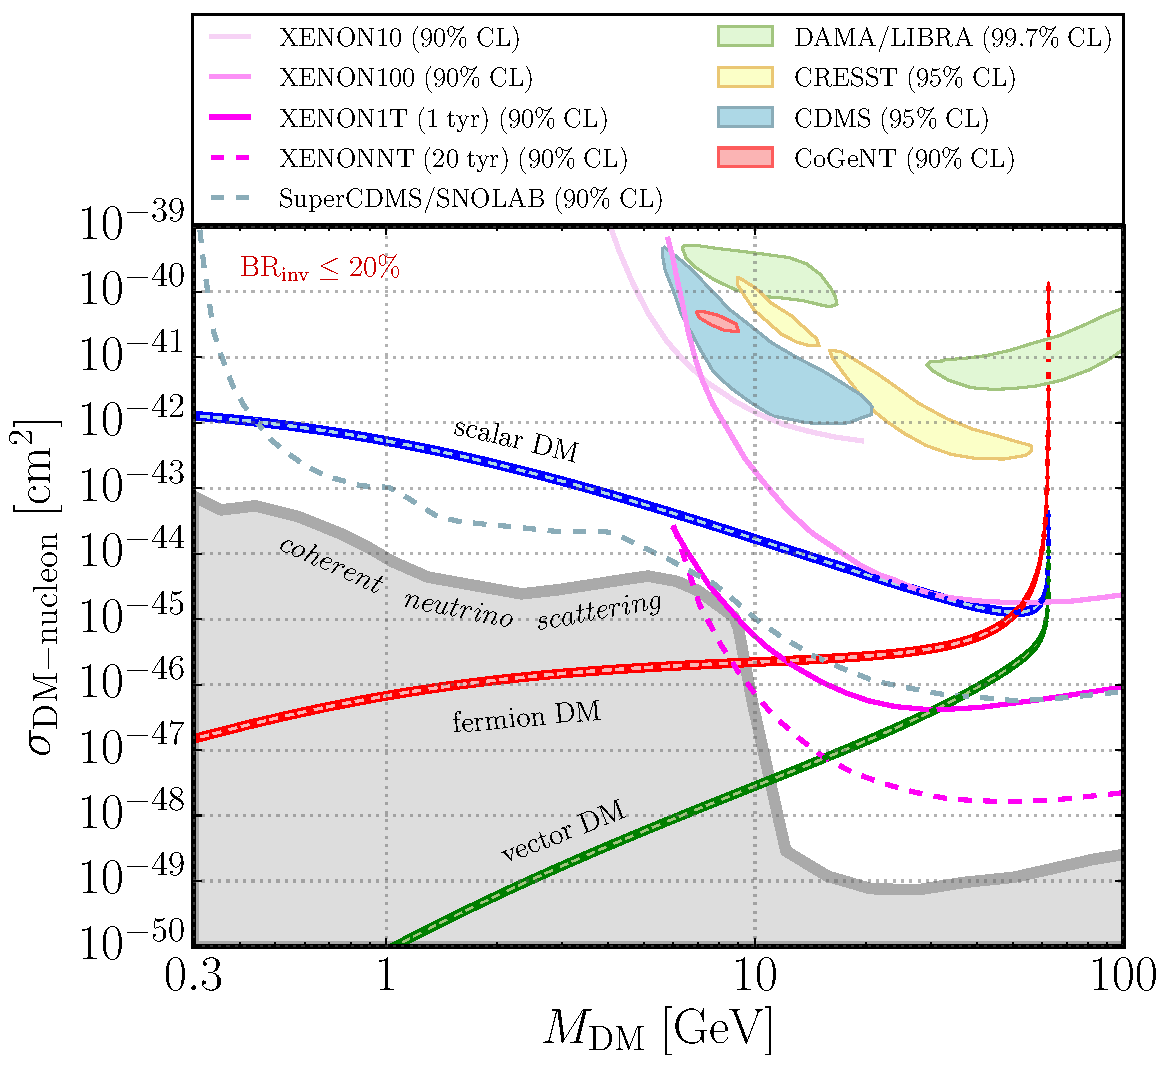
\includegraphics[width=0.49\textwidth]{\main/section6/plots/DM-SI-XS_HiggsPortalDM_BRinv_0p2_HoferichterF}
\hfill
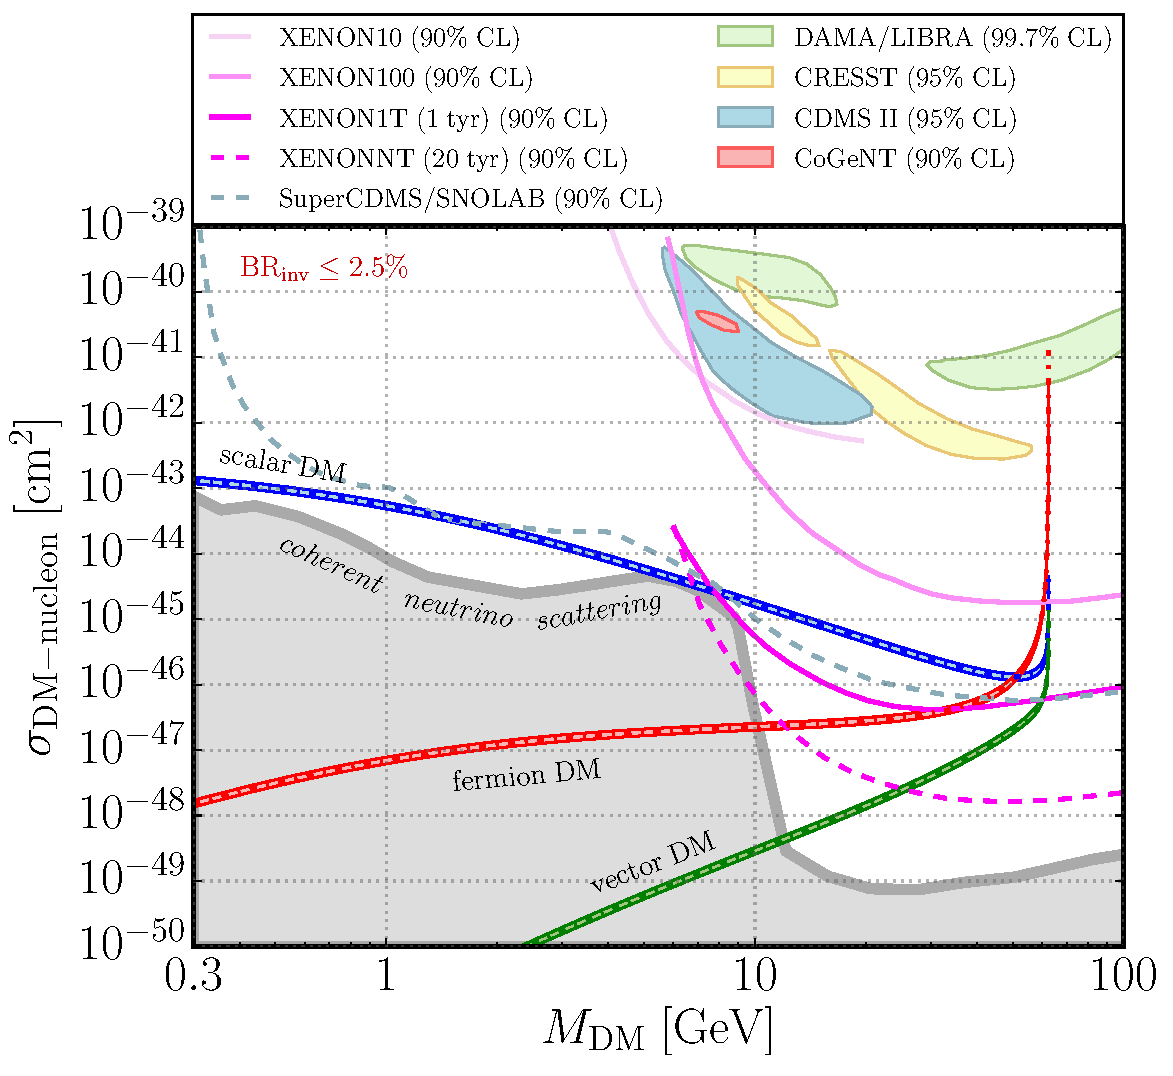
\includegraphics[width=0.49\textwidth]{\main/section6/plots/DM-SI-XS_HiggsPortalDM_BRinv_0p025_HoferichterF}
\caption{\label{fig:mini} Implications for the minimal Higgs portal model: Comparison of current (\emph{left figure}) and future HL-LHC (\emph{right figure}) limits from invisible Higgs searches  with limits from DM direct detection experiments on the spin-independent DM-nucleon scattering cross section, $\sigma_{\mathrm{DM}-\mathrm{nucleon}}$, as a function of the DM mass, $\MDM$. The inferred limits from invisible Higgs searches are shown for scalar DM (\emph{blue curve}), fermion DM (\emph{red  curve}) and for vector DM (\emph{green  curve}). In addition we show present limits (\emph{solid lines}), favoured regions (\emph{filled areas}) and future sensitivity (\emph{dashed lines}) of the DM direct detection experiments \textsc{Xenon10}~\cite{Angle:2011th}, \textsc{Xenon100}~\cite{Aprile:2012nq}, \textsc{Xenon1T}~\cite{Aprile:2018dbl}, \textsc{XenonNT}~\cite{Aprile:2015uzo}, \textsc{SuperCDMS} at SNOLAB~\cite{Agnese:2016cpb}, \textsc{DAMA/LIBRA}~\cite{Savage:2008er}, \textsc{Cresst}~\cite{Angloher:2011uu}, \textsc{CDMS~II}~\cite{Agnese:2013rvf} and \textsc{CoGeNT}~\cite{Aalseth:2012if} (\emph{see legend}). The grey area indicates regions inaccessible to DM direct detection experiments due to the irreducible neutrino flux background~\cite{Billard:2013qya}.}
\label{fig:minimalHP}
\end{figure}



\subsubsection{Scalar singlet portal}
\label{sec6:singletHP}
We now turn our discussion to a model that features an additional scalar singlet in the visible sector, which provides the portal interaction to the hidden DM sector. In contrast to the minimal Higgs portal discussed in Section~\ref{sec6:minimalHP}, this model allows for a modification of the $125\UGeV$ Higgs couplings, and thus for a non-trivial interplay between direct invisible Higgs searches and Higgs rate measurements at the HL-LHC. For illustration, we focus here on the case of scalar DM, the other cases (fermion and vector DM) can be treated analogously. The model is inspired by Refs.~\cite{Englert:2011yb,Robens:2015gla}.



The SM Higgs sector is extended by two real scalar singlet fields, $S$ and $X$. Imposing a $\mathbb{Z}_2$ symmetry described by the transformation $S\to -S$, $X\to -X$, the model is characterised by the scalar potential $\mathcal{V} = \mathcal{V}_\mathrm{visible}  + \mathcal{V}_\mathrm{hidden}$, where
\begin{align}
\label{Eq:Vvis}\mathcal{V}_\mathrm{visible} &=   \mu_{\Phi}^2 \Phi^\dagger \Phi + \lambda_\Phi (\Phi^\dagger \Phi)^2 + \mu_S^2 S^2 + \lambda_S S^4 + \lambda_{\Phi S} \Phi^\dagger \Phi S^2,\\
\label{Eq:Vhid} \mathcal{V}_\mathrm{hidden} &= \frac{1}{2}\left[\mu^2_{X} X^2 + \lambda_X X^4 + \lambda_{SX} S^2 X^2 + \lambda_{\Phi X} \Phi^\dagger \Phi X^2\right]. 
\end{align}
For the sake of simplicity we assume that the quartic interaction between the scalar doublet $\Phi$ and the DM scalar $X$ can be neglected, $\lambda_{\Phi X} \approx 0$. After electroweak symmetry breaking the scalar $\mathrm{SU}(2)_L$ doublet field $\Phi$ is given by 
$\Phi \equiv \left(0 \quad \phi + v\right)^T/\sqrt{2}$, with the vacuum expectation value (VEV) $v \approx 246\UGeV$. 
We assume the scalar field $S$ to acquire a non-zero VEV, $v_S$, which softly breaks the $\mathbb{Z}_2$ symmetry, such that the singlet field $S$ is given by $S \equiv (s + v_S)/\sqrt{2}$. Through the last term in Eq.~\eqref{Eq:Vvis} the non-zero VEVs induce a mixing of the physical degrees of freedom of these two fields, $\phi$ and $s$,
\begin{align}
\begin{pmatrix} h \\ H \end{pmatrix} = \begin{pmatrix} \cos \alpha & -\sin\alpha \\ \sin\alpha & \cos\alpha \end{pmatrix} \begin{pmatrix} \phi \\ s \end{pmatrix},
\end{align}
with the masses of the physical states $h$ and $H$ given by
\begin{align}
M_{h/H}^2 = \lambda_\Phi v^2 + \lambda_S v_S^2 \mp \sqrt{\left(\lambda_\Phi v^2 - \lambda_S v_S^2\right)^2 + \left(\lambda_{\Phi S} v v_S\right)^2},
\end{align}
and the mixing angle $\alpha \in [-\tfrac{\pi}{2}, \tfrac{\pi}{2}]$ given by
\begin{align}
\tan 2\alpha = \frac{\lambda_{\Phi S} v v_s}{\lambda_S v_S^2 - \lambda_\Phi v^2}.
\end{align}
In contrast, $X$ does not acquire a VEV. As a result $X$ is stable and thus a possible DM candidate, with a mass given by
$M_X^2  = \mu_X^2  + \lambda_{SX} v_S^2/2$.

In this analysis, we assume $M_H = 125.09\UGeV$, and $M_h < M_H$. Furthermore, we discard the quartic interaction term $\propto \lambda_X$ in Eq.~\eqref{Eq:Vhid} as this operator is irrelevant for our study. With this, the model can then be parametrised in terms of the following input quantities:
\begin{align}
M_h, \cos\alpha, v_S, M_X, \lambda_{SX}.
\end{align}
The couplings of the Higgs bosons $h$ and $H$ to SM gauge bosons and fermions are universally suppressed by the mixing,
\begin{align}
g_h/g_{h,\mathrm{SM}} = \cos \alpha , \qquad g_H/g_{H,\mathrm{SM}} = \sin\alpha.
\end{align}
If the DM scalar $X$ is light enough the portal coupling $\lambda_{SX}$ gives rise to decays of the Higgs bosons $h$ and $H$ to the invisible $XX$ final state. The partial decay widths are given by
\begin{align}
\label{eq:invdecaywidth}
\begin{array}{l} \Gamma(h\to XX) = \sin^2\alpha \cdot \Gamma_{XX} (M_h), \\ \Gamma(H\to XX) = \cos^2\alpha \cdot \Gamma_{XX} (M_H), \end{array} \quad \mbox{with} \quad \Gamma_{XX}(M) = \frac{\lambda_{SX}^2 v_S^2 }{32\pi M} \sqrt{1 - \frac{4M_X^2}{M^2}}.
\end{align}
Furthermore, if $M_h \le M_H/2$, the heavier Higgs boson $H$ can decay into $hh$, with the partial width given by
\begin{align}
\Gamma(H\to hh) = \frac{\lambda_{Hhh}^2}{32\pi M_H} \sqrt{1 - \frac{4M_h^2}{M_H^2}},
\end{align}
and the effective $Hhh$ coupling\footnote{Note that the relative sign between the two terms in Eq.~\eqref{Eq:lamHhh} differs with respect to Eq.~(13) in Ref.~\cite{Englert:2011yb}.}
\begin{align}
\label{Eq:lamHhh}
\lambda_{Hhh} = & - 3\sin2\alpha \left[ \lambda_S v_S \sin\alpha  + \lambda_{\Phi} v \cos\alpha \right] \nonumber\\
& - \tan2\alpha \left( \lambda_S v_S^2 - \lambda_{\Phi} v^2 \right) \left[ (1-3\sin^2\alpha) \frac{\cos\alpha}{v} + (1-3 \cos^2\alpha) \frac{\sin\alpha}{v_S} \right].
\end{align}


Through the successive decay of the lighter Higgs boson $h$ into either final states with SM particles (denoted as `SM') or the invisible $XX$ final state, this gives rise to the following signatures\footnote{{Note that LHC searches for the semi-invisible and visible final states are highly complementary to invisible Higgs searches in this model.}}
\begin{align}
H \to hh \to \left\{ \begin{array}{l} (\mathrm{SM}) (\mathrm{SM}) ,\quad \mbox{(visible)}, \\ (\mathrm{SM}) (XX) ,\quad \mbox{(semi-invisible)}, \\
(XX) (XX) ,\quad \mbox{(invisible)}.
\end{array} \right.
\end{align}

The branching ratio of the invisible decay of the SM-like Higgs boson $H$ is given by
\begin{align}
\BRHinv = \mathrm{BR}(H\to XX) + \mathrm{BR}(H\to hh) \cdot \mathrm{BR}(h\to XX)^2.
\end{align}
 
\begin{figure}[t]
\centering
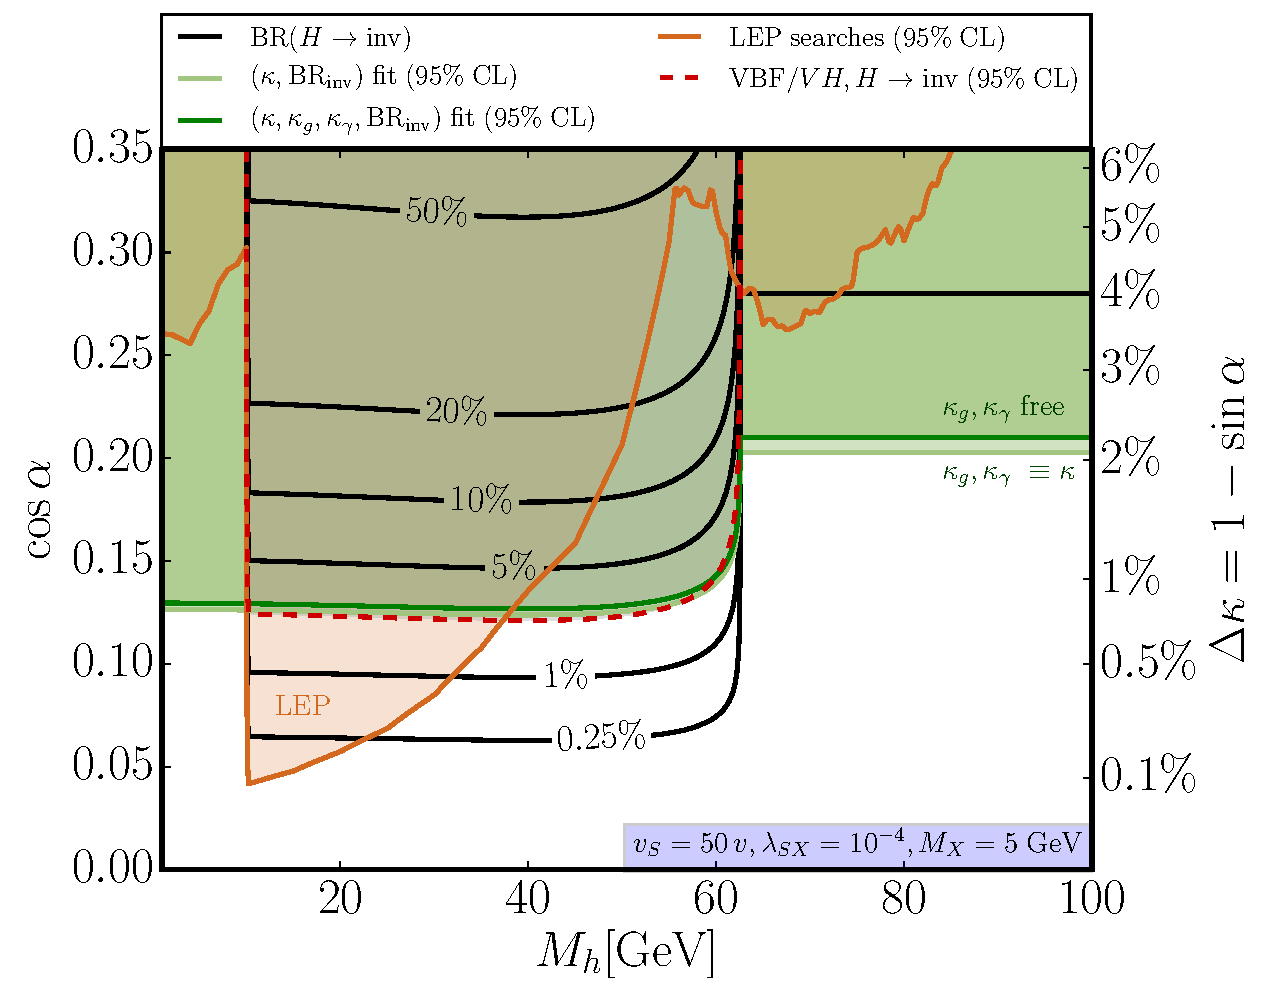
\includegraphics[width=0.5\textwidth]{\main/section6/plots/mh_cosa_vs50vH_lamSX0p0001_MX5GeV_LEPBRinvkunikgga}\hfill
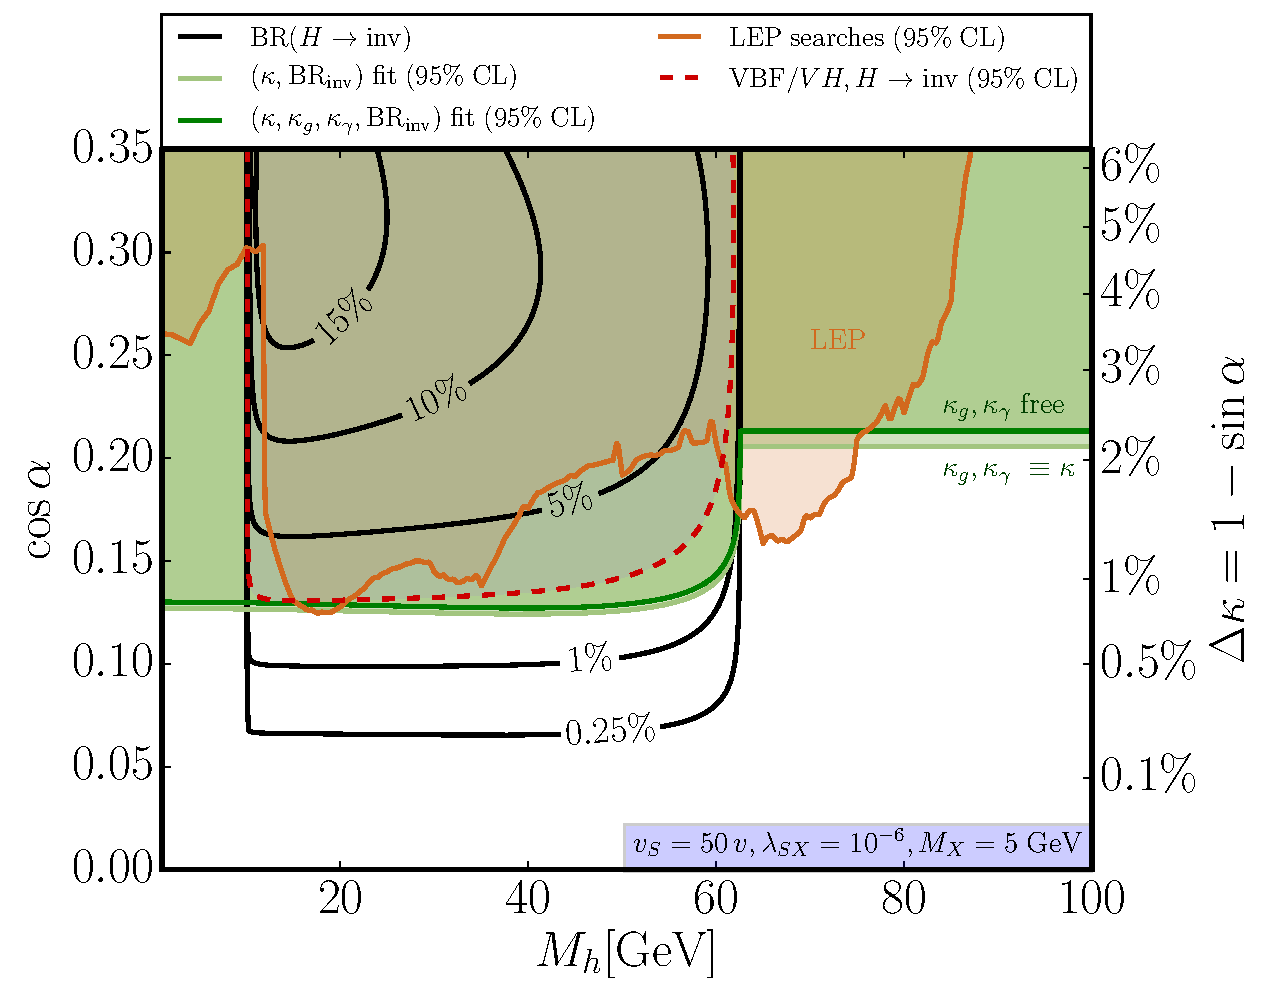
\includegraphics[width=0.5\textwidth]{\main/section6/plots/mh_cosa_vs50vH_lamSX0p000001_MX5GeV_LEPBRinvkunikgga}\\
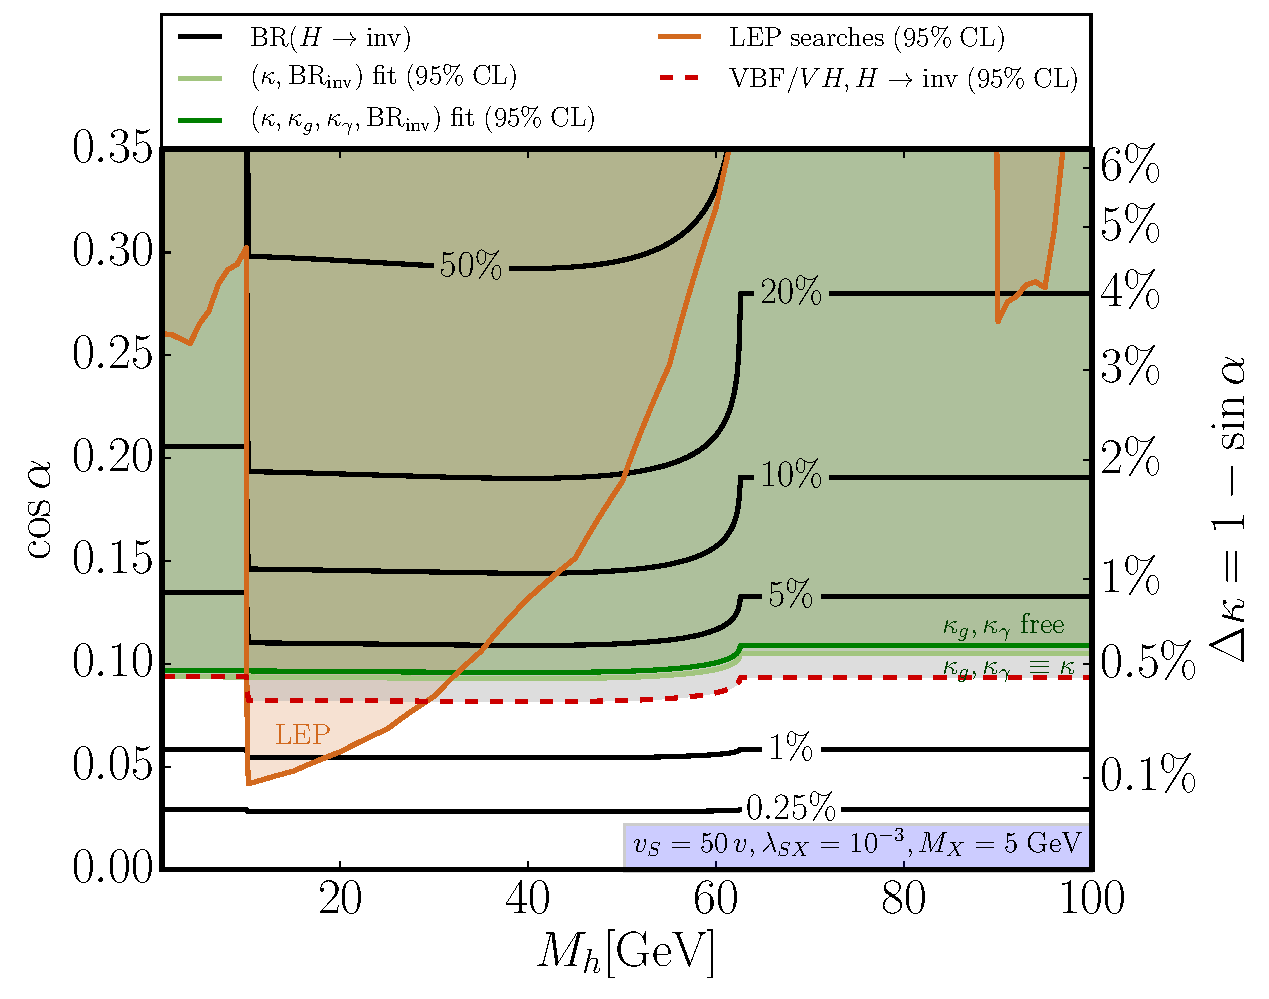
\includegraphics[width=0.5\textwidth]{\main/section6/plots/mh_cosa_vs50vH_lamSX0p001_MX5GeV_LEPBRinvkunikgga}\hfill
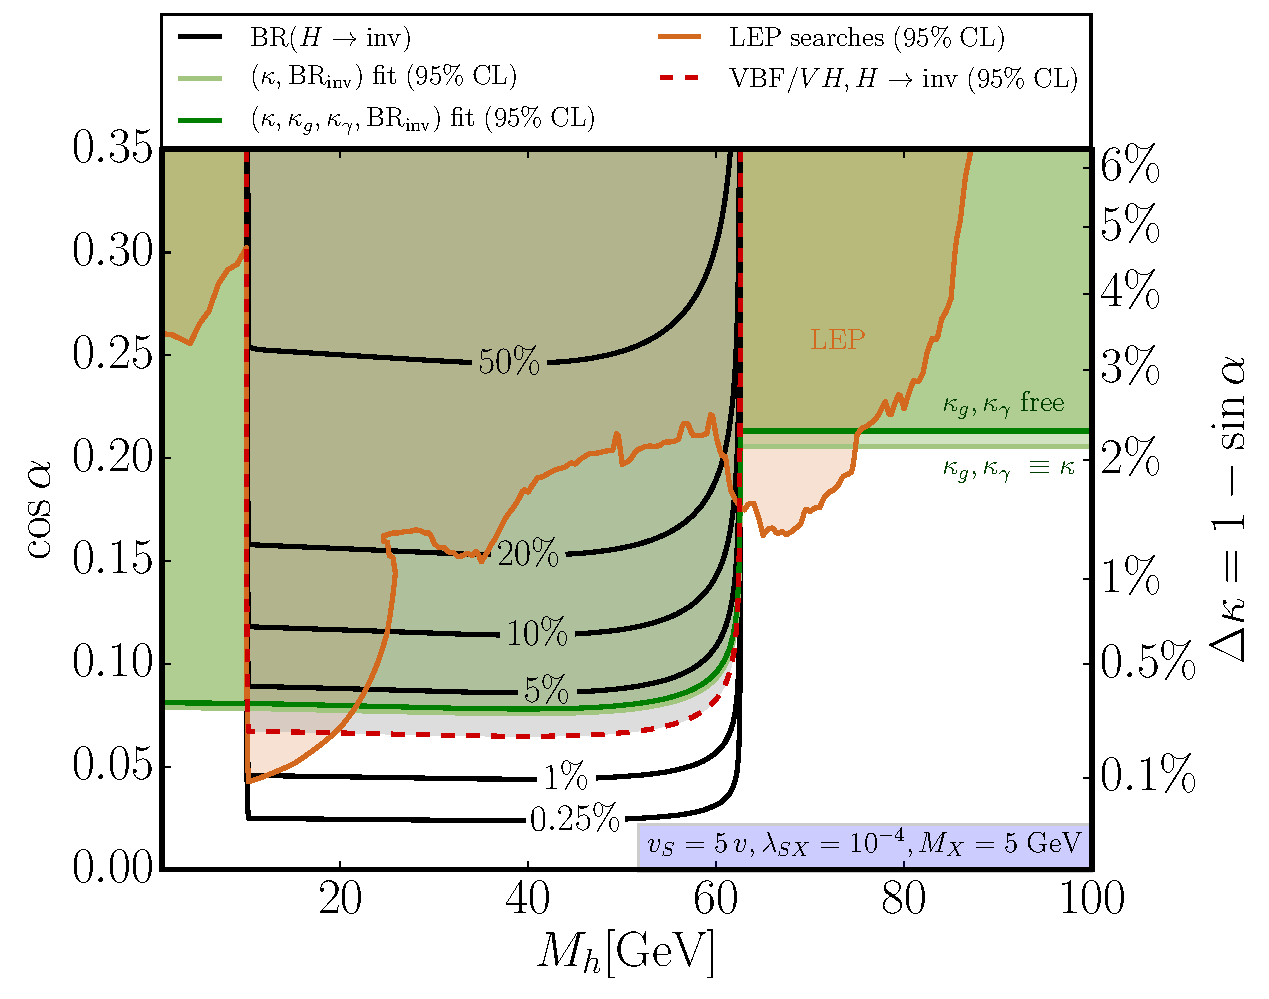
\includegraphics[width=0.5\textwidth]{\main/section6/plots/mh_cosa_vs5vH_lamSX0p0001_MX5GeV_LEPBRinvkunikgga}
\caption{Implications for the scalar singlet portal model, shown in the $(M_h, \cos\alpha)$ parameter plane for a DM mass of $M_X = 5\UGeV$ and $(v_S, \lambda_{SX}) = (50\,v, 10^{-4})$ [\emph{top left}], $(50\,v, 10^{-6})$ [\emph{top right}], $(50\,v, 10^{-3})$ [\emph{bottom left}] and $(5\,v, 10^{-4})$ [\emph{bottom right}]. Black solid contours show the invisible Higgs decay rate, $\mathrm{BR}(H\to \mathrm{inv})$, the red dashed contour/grey area indicates the expected HL-LHC limit from invisible Higgs searches, pale and bright green contours/areas indicate the indirect constraints from HL-LHC Higgs rate measurements (using the two parametrisations, see Section~\ref{sec6:effC}), and the orange contour/area marks the excluded region from LEP searches. See text for more details.}
\label{Fig:singletportal}
\end{figure}
 
 In Fig.~\ref{Fig:singletportal} we show the invisible Higgs decay rate $\BRHinv$ in the $(M_h, \cos\alpha)$ plane, for fixed DM mass $M_X = 5\UGeV$, and four choices $(v_S, \lambda_{SX}) = (50\,v, 10^{-4})$ [\emph{top left}], $(50\,v, 10^{-6})$ [\emph{top right}], $(50\,v, 10^{-3})$ [\emph{bottom left}] and $(5\,v, 10^{-4})$ [\emph{bottom right}]. For better illustration, the secondary y-axis shows the deviation from the SM coupling strength, $\Delta \kappa = 1 -\sin\alpha$, of the heavier Higgs boson $H$. The $\BRHinv$ prediction is given by the black solid contours. Various constraints (at $95\%\CL$) are included in the figures: future direct invisible Higgs searches (\emph{red dashed contour}/\emph{grey area}), future indirect limits from Higgs rate measurements {at the HL-LHC (assuming S2)} using the two parametrisations of Section~\ref{sec6:effC} [cf.~Fig.~\ref{fig:effC}] (\emph{solid pale/bright green contour and area}), and LEP searches for the lighter Higgs boson $h$ (\emph{orange contour and area}), obtained via \texttt{HiggsBounds}~\cite{Bechtle:2008jh,Bechtle:2011sb,Bechtle:2013wla}. For the latter, the relevant experimental analyses are searches for $e^+e^-\to Zh$ production with $h$ either decaying to invisible particles~\cite{Searches:2001ab,Abdallah:2003ry,Achard:2004cf,Abbiendi:2007ac} or to SM particles (in particular, $b\bar{b}$)~\cite{Schael:2006cr}, as well as the decay mode independent analysis by OPAL~\cite{Abbiendi:2002qp}.



In all four panels of Fig.~\ref{Fig:singletportal} we can identify two kinematic thresholds for the invisible $H$ decay: at $M_h = M_H/2 \simeq 62.5\UGeV$, where the cascade decay $H\to hh\to (XX)(XX)$ becomes available for decreasing $M_h$, and at $M_h = 2 M_X = 10\UGeV$, where the decay $h\to XX$ kinematically closes for smaller $M_h$, and thus the $H\to hh$ decay cannot further lead to an invisible final state. Above the first threshold, $M_h > M_H/2$, and below the second threshold, $M_h < 2M_X$, the invisible $H$ decay is solely given by {the direct decay} $H\to XX$. 

For the parameter choice $(v_s, \lambda_{SX}) = (50\,v, 10^{-4})$ (\emph{top left panel}), the direct invisible Higgs searches at the HL-LHC {will} provide similar bounds as the indirect constraints from the Higgs rates for the mass range $M_h \in [2 M_X, M_H/2]$. However, in the mass range $M_{h}\sim (10-40)\UGeV$, the LEP searches for invisible $h$ decays will still yield the strongest exclusion. Note that the Higgs rate measurements are always constraining the sum $\BRNP = \mathrm{BR}(H\to XX) + \mathrm{BR}(H\to hh)$, regardless of whether the decay $H\to hh$ leads to an invisible final state. Hence, they remain to be sensitive in the low mass region $M_h < 2 M_X$.

For a larger Higgs-portal interaction, $\lambda_{SX} = 10^{-3}$ (\emph{bottom left panel}), the direct decay $H\to XX$ becomes more prominent, leading to sizeable $\BRHinv$ even at smaller $\cos\alpha$. Here, direct invisible Higgs searches at HL-LHC will be most constraining and will supersede the LEP limits except in the mass range $M_h\sim (10-33)\UGeV$. {In contrast,} for very small Higgs-portal interaction, $\lambda_{SX} = 10^{-6}$ (\emph{top right panel}) {the invisible Higgs decay rates are much smaller. Nevertheless,} future indirect constraints from Higgs rate measurements will supersede the LEP limits {in almost the entire mass range except for $M_h$ values between $62$ to $75\UGeV$.}
Note that the LEP exclusion arises from $e^+e^- \to Zh \to Z(b\bar{b})$ searches~\cite{Schael:2006cr}.

If we decrease the VEV of the singlet field, $v_s = 5\,v$ (\emph{bottom right panel}), the effective $Hhh$ coupling becomes larger, leading to a more pronounced $H\to hh$ decay if kinematically accessible. Hence, in the region $M_{h} < M_H/2$, the HL-LHC constraints both from direct invisible Higgs searches and Higgs rate measurements are very strong and supersede the LEP constraints in almost the entire mass range up to $M_h \lesssim M_H/2$. {In this case, the direct invisible Higgs searches} are slightly more {sensitive} than the {Higgs rate measurements}.

In summary, the example parameter choices made in Fig.~\ref{Fig:singletportal} illustrate an interesting interplay between past LEP searches for a light Higgs boson $h$, future HL-LHC searches for an invisibly decaying SM-like Higgs boson $H$, and future HL-LHC precision Higgs rate measurements. Depending on the parameter choice, each experimental probe can be the most sensitive/constraining one, which highlights their complementarity and strongly motivates a corresponding experimental program at the HL-LHC. 



%%%%%%%%%%%%%%%%%%%%%%%%%%%%%%%%
\subsection{Conclusions}
\label{sec6:conclusions}
%%%%%%%%%%%%%%%%%%%%%%%%%%%%%%%%

Higgs portal models are intriguing and simple new physics scenarios that contain a dark matter candidate which can be tested at collider as well as astrophysical experiments. The HL-LHC will be able to constrain the Higgs boson--dark matter coupling constant and probe the parameter regime down to an invisible Higgs decay rate of 2$\%$. For low dark matter masses, $M_\text{DM}\,\lesssim\,30\UGeV$, these bounds are typically more constraining than limits obtained from dark matter direct detection experiments. For a specific model with two visible scalar states and a scalar dark matter candidate, we presented scenarios for which future HL-LHC {searches} will supersede complementary constraints from LEP searches for a light scalar boson. In summary, the future HL-LHC measurements of the Higgs signal strength, as well as {direct searches} for the invisible decay of the observed Higgs boson, promise to provide important insight within the framework of Higgs portal models. {The sensitivity can further be improved by the future electron-proton collider LHeC. In particular, the indirect constraints from Higgs rate measurements will improve substantially if HL-LHC and LHeC results are combined.}




\end{document}
